% Requesting draft will show any overfull boxes when the document is compiled. Should be black lines on the document where the boxes are overfull.
\documentclass{refrep}

% For increasing the width of the left margin.
\setlength{\marginparwidth}{5.75cm}
% For adding minimum space between notes in the left margin.
\setlength{\marginparpush}{0.25cm}

\usepackage{todonotes}

% These packages are used for typing inline Python code and for fixing some of the weird things that listings does with single- and double-quote characters.
% https://tex.stackexchange.com/questions/166790/how-can-i-get-straight-double-quotes-in-listings
\usepackage[T1]{fontenc}
\usepackage{textcomp}
\usepackage{listings}
\lstset{upquote=true, showstringspaces=false}

\usepackage[utf8]{inputenc}
%Commented these out b/c they don't seem to be necessary to put a caption beneath tables. if the spacing gets messed up, try un-commenting them.
%\usepackage{caption}
%\captionsetup[table]{position=bottom}
\usepackage{url}
\usepackage{graphicx}  % This package lets you import images into the document.
\graphicspath{ {BioPype_images/} }  % Specify the path to the folder where the images will be imported from.
\usepackage[toc,page]{appendix}

% This is to stop the individual appendix entries from appearing in the ToC.
\usepackage{etoolbox}
\appto\appendix{\addtocontents{toc}{\protect\setcounter{tocdepth}{0}}}
% reinstate the correct level for list of tables and figures
\appto\listoffigures{\addtocontents{lof}{\protect\setcounter{tocdepth}{1}}}
\appto\listoftables{\addtocontents{lot}{\protect\setcounter{tocdepth}{1}}}

\usepackage{hyperref}  % Allows hyperlinks.

% For making gray text boxes
\usepackage[tikz]{bclogo}
\definecolor{vlightgray}{gray}{0.90}

% For bibliography
\usepackage{natbib}
\bibliographystyle{apalike}

% For letting underlined text wrap to the next line when it reaches the edge of the page.
\usepackage{soul}

\maxipagerulefalse

\title{BioPype: A crash course in bioinformatics and custom pipelines}

\author{Ethan Gniot}
\date{May 2018}

\begin{document}


\maketitle 
\listoftodos
\tableofcontents % This creates the table of contents; autofills Chapters, sub-chapters (aka "sections"), and page numbers.

% Add an asterisk before the {} to make an un-numbered chapter that won't be included in the ToC.
\chapter{Foreword}

\section{Goal}
This tutorial aims to improve your general understanding of bioinformatics through several methods:
\begin{itemize}
    \item Define technical terms commonly used in bioinformatics methods and found in the literature.
    \item Provide a collection of various useful resources, including...
    \begin{enumerate}
        \item Resources for finding tools, data, and background information that can help answer your research questions.
        \item Resources that explain details about bioinformatics concepts and techniques in beginner-friendly language.
    \end{enumerate}
    \item Demonstrate how Python can be used to answer your research questions by combining existing bioinformatics tools and automating repetitive or time-consuming tasks.
\end{itemize}

\section{How to use this book}
The main text of this book is written in the right-hand margin. The left-hand margin contains special markers and important notes to the reader. Most reference materials are consolidated in the appendices at the end of the book. The book can be used as a self-paced tutorial with the help of the markers described below.

------------------------------- 

\textit{Lorem ipsum dolor sit amet, consectetur adipiscing elit. Maecenas eu felis sodales, interdum purus nec, interdum ex. Integer at nunc \marginlabel{This is a margin label. I will write things here to further explain the main text, define jargon, etc.} ultricies, tempus nibh eget, egestas risus. Suspendisse aliquam, lorem at dictum accumsan, dolor elit euismod velit, a gravida risus libero non felis. Donec a tortor tempor, scelerisque sapien posuere, volutpat erat. Morbi in imperdiet velit. Vivamus sagittis, massa sit amet venenatis euismod, elit eros aliquam diam, molestie faucibus lectus nisi euismod erat. Nulla id dictum mi.}

\attention \textbf{The arrow that points to this line is an "Attention" marker. It will indicate key pieces of information that you should pay special attention to.} \textit{Curabitur egestas aliquam nisl, pharetra finibus mauris placerat nec. Nam in diam risus. Nulla mollis purus quis feugiat tristique. Vestibulum et sollicitudin ante, at sagittis ipsum. Nunc hendrerit ante sed massa semper eleifend.}

\seealso{This kind of annotation will reference appendix entries that you can consult for more-detailed information about the main text.} Ut ultrices eros velit, at faucibus ante rutrum eget. Pellentesque a molestie diam. Curabitur mattis dui a risus lacinia fringilla. Phasellus porttitor elit nec neque euismod, id ultrices elit lobortis. Aliquam molestie sem. Curabitur sit amet urna faucibus, vulputate arcu sit amet, fermentum ipsum. Nulla facilisi. Nam ullamcorper eget leo id malesuada.


\section{Source Code}
The source code for this manual, the accompanying tutorial, and the BioPype package can all be found at \url{github.com/EthanGniot/BioPype}.


\section{Pre-requisites}
\subsection*{Computer requirements}
\begin{itemize}
    \item At least 4GB RAM minimum.* 16GB RAM if possible (the more RAM, the better)
    \begin{itemize}
    \item *At 4GB RAM, one step of the BioPype analysis takes \~2.5 hours to finish when analyzing 20 samples. With less RAM, expect the process to take longer. Conversely, more RAM will increase the speed of the analysis. 
    \end{itemize}
    \item BioPype was developed and tested using a MacBook Pro (Retina, 13-inch, Late 2013) running macOS 10.13.4 High Sierra. BioPype should be compatible with similar macOS versions, as well as Linux, though it has not yet been tested on Linux.
    \item Storage requirements will vary depending on the amount of data you intend to analyze. The analysis performed in this tutorial required at least 500GB and were satisfied by using a 2TB external hard drive.
\end{itemize}


%
%\chapter{Sample Information}

%While we are building the BioPype pipeline, we will need a dataset that we can use to test our pipeline throughout the process and make sure it is working as intended. In order to do this, we must use a dataset that's already been analyzed so that we know what the results should look like. When we test our pipeline, if our results match the results of the original analysis, then we will know that our tool is working correctly.

%There are several test datasets available to us for testing the feature that analyzes the relative abundance of bacteria in the microbiota.

%The first is the dataset used in both the QIIME ``Illumina Overview Tutorial" (\ref{appendix:IlluminaOverTut}) and the QIIME 2 ``Moving Pictures" tutorial (\ref{appendix:MovingPicTut}) derived from the \textit{Moving Pictures of the Human Microbiome} study, where two human subjects collected daily samples from four body sites: the tongue, the palm of the left hand, the palm of the right hand, and the gut (via fecal samples obtained by swapping used toilet paper) \cite{Caporaso2011}. These data were sequenced using the barcoded amplicon sequencing protocol described in \textit{Global patterns of 16S rRNA diversity at a depth of millions of sequences per sample} \cite{Caporaso2011a}. A more recent version of this protocol that can be used with the Illumina HiSeq 2000 and MiSeq can be found here.

%\chapter{Setting the scene}
%    \label{chap:scene}
%("Here" is a hypothetical situation/research question that a student may have. This is the research question that will be answered by the pipeline we are creating.)

\chapter{Microbiome Analysis}
The analysis used in this tutorial will focus on analysis of the human gut microbiome, but BioPype can be used to analyze the microbiomes of other communities as well.
\section{The Gut Microbiome}
%
\seealso{\footnotesize For more explanation about the \textbf{gut microbiota} and \textbf{gut microbiome}, see \ref{appendix:microbiome-vs-microbiota}.}
%
The human gut is home to trillions of microbes. The collection of physical micro-organisms that live in the gut is referred to as the \textbf{gut microbiota}. The \textbf{gut microbiome} refers to all of the genes contained within these micro-organisms, as well as their functions and interactions.

%
Human microbiota can play host to many different kinds of microbes, including bacteria, archaea, and fungi. For the sake of this tutorial, we are going to focus on the role of bacteria in human microbiomes.

\marginlabel{\footnotesize \textbf{Gut dysbiosis:} deviation from "normal" gut microbiota composition.}
Sometimes the biodiversity of the gut is thrown out of balance. When the composition of the microbiota is significantly altered, and bacterial populations that normally compose a large percentage of the microbiota become underrepresented (or underrepresented populations become overrepresented), the gut is in a state of \textit{dysbiosis}.
%
\seealso{\footnotesize For an approachable overview of the human microbiome, the effects of microbiome variation on human health and disease, and important research questions regarding the microbiome, see \cite{Cho2012}.}
%
 \textbf{Gut dysbiosis} is important to study because it has been implicated in many physical and neurological human health conditions, including diabetes, rheumatoid arthritis, Alzheimer's, inflammatory bowel disease (IBD), colon cancer \citep{Buford2017, Kennedy2014, Castellarin2012},  chronic fatigue syndrome \citep{Lakhan2010}, obesity \citep{Turnbaugh2006,Turnbaugh2009}, bacterial vaginosis \citep{Africa2014}, ulcerative colitis {\citep{Mandal2015, Matsuoka2015}, anxiety, and depression \citep{Evrensel2015, Lach2018}
%
\section{Relative Abundance Analysis}
%
\marginlabel{\footnotesize \textbf{Relative abundance} is a measure of how common or rare a taxon is, relative to other taxa in its community, and is usually expressed as a percentage. For more information on \textbf{relative abundance} analyses, see Appendix \ref{appendix:abundance-analyses}.} 
%
BioPype lets users examine the \textbf{relative abundance} of bacterial taxa in each experimental sample. Relative abundance analyses help visualize the structure of the micro-organism community. Users can use BioPype to analyze bacterial \textbf{amplicon} sequencing data to determine which micro-organisms are present and in what proportion.
%
\seealso{\footnotesize For information on \textbf{amplicon} sequencing vs. shotgun sequencing, see Appendix \ref{appendix:amplicon}.}
%
The idea is to take the sequences from a gut sample and assign them to a taxon. To do that, we group (or cluster) sequences based on their similarity to define \textbf{Operational Taxonomic Units (OTUs)}. 
%
\marginlabel{\footnotesize \textbf{Operational Taxonomic Unit (OTU)}: A group of sequences that share significant similarity based on some marker gene. Groups can be treated as a single taxon (e.g., genus, species, etc. depending on the clustering threshold) for analysis purposes. For more info, see Appendix \ref{appendix:otu}.}
%
Using the number of sequences assigned to each OTU/taxon, BioPype can determine the relative abundance of each micro-organism in a sample and plot the results on an interactive bar chart.

For example, studies have found that the genera \textit{Bacteroides} and \textit{Lactobacillus} are both prevalent in the healthy human gut microbiome, but \textit{Bacteroides} has a higher relative abundance than \textit{Lactobacillus} \cite{Lloyd-Price2016}. In other words, out of all the sequences obtained from a healthy human gut sample, a larger percentage of those sequences will be assigned to the \textit{Bacteroides} OTU than to the \textit{Lactobacillus} OTU during a relative abundance analysis. 

Relative abundance is an important measure of biodiversity in the gut. Using BioPype to perform a relative abundance analysis allows examination of gut biodiversity at 7 different taxonomic levels, which helps identify instances of gut dysbiosis in research subjects. 

\section{Metagenomics}
\attention{\textit{THIS FUNCTIONALITY HAS NOT BEEN COMPLETED YET, BUT WILL BE ADDED IN FUTURE UPDATES}}

BioPype can also be used to predict which genes are present in microbiome samples. From these predicted genes, users can do two things. 

First, they can generalize the functions encoded across all bacteria that are present in an experimental condition's microbiome (i.e., at the metagenomic scale) and visualize the relative distribution of these functions with a bar chart. Having this functional snapshot of a metagenome is useful because a functional overview of the experimental condition can be compared to a functional overview of the control condition to see if there are differences in the two groups' functional capabilities. When comparing the microbiomes of disordered vs. non-disordered samples, having a visual depiction of the differences in functional capabilities can make it easier to find the cause of the disorder by narrowing down the potential sources of the condition. 

For example, certain G protein-coupled receptors (GPCRs) in the gut are associated with some of the diseases associated with gut dysbiosis, such as inflammatory bowel disease (IBD) \citep{Cohen2017}. Research has also shown that bacteria interact with their environment via the release of small molecules \citep{Li2012}. From these premises, one could hypothesize that IBD may be caused by the over-production of certain effector molecules from the gut microbiome. This hypothesis may be tested by using BioPype to compare the functional capabilities of the IBD microbiome with that of a healthy control microbiome. If the results show, for example, that the IBD gut metagenome has a greater proportion of genes associated with lipid production than the control metagenome, it indicates potential support for the user's hypothesis. They can now refine their investigation by narrowing the scope of their search to only analyze genes associated with lipid synthesis.

Second, users can use BioPype to predict the functions of \textit{individual} genes. This is useful because it allows users to identify a specific gene of interest for their research question, which they can then design a validation experiment for. 

Continuing with our above example hypothesis about the gut microbiome's role in IBD, the user can now turn their focus to the functions of specific lipid-synthesis genes that are being overrepresented in IBD patients' microbiomes. Upon examining the functions of individual genes, they find that N-acyl amide synthase genes are enriched in the IBD microbiome. Wet-lab validation experiments will confirm that the lipids encoded by these genes are able to interact with GPCRs that regulate GI tract physiology \citep{Cohen2017}. This suggests that these lipids, and their associated genes in the microbiome, have the potential to cause IBD during times of dysbiosis by activating GPCRs in the gut \citep{Cohen2017}, thus supporting the user's original hypothesis. Additionally, one can use these findings to focus future research questions about the role of the human microbiome in health disorders by searching for correlations between N-acyl amide synthase genes and other conditions. For instance, since the products of these genes interact with GPCRs to potentially regulate IBD, and IBD is associated with anxiety and depression, investigation may reveal that the interaction between these genes and GPCRs potentially regulate anxiety and depression as well.

%
\section{Python}
To make use of this tutorial and the BioPype package, you will need to be familiar with the basics of the Python coding language. The free DataCamp course \textit{Intro to Python for Data Science} (\url{https://www.datacamp.com/courses/intro-to-python-for-data-science?tap_a=5644-dce66f&tap_s=116411-750171}) is a quick and easy introduction to the basics of the language. It covers:
%
\begin{itemize}
\item Variables and variable assignment
\item Basic data types (strings, integers, floats, lists, booleans, ) and converting between types
\item Calculations with variables
\item Functions and arguments
\item The \verb|help()| function.
\item Methods
\item Packages and importing packages
\item The basics of the NumPy package (The material covered in the NumPy chapter of the DataCamp tutorial is not required for using BioPype, but if you are new to Python,  it's a great way to practice/apply the concepts they teach you in Chapters 1-3.)
\end{itemize}
%
The DataCamp course should take \~4 hours to complete (less, if you forego NumPy chapter), and will teach you everything you'll need to know about Python in order to make use of BioPype. 

If you decide that you'd like to start creating your own tools with Python, there's a bit more you'll need to know. Resources for learning how to create your own functions, classes, packages, and more can be found in Appendix \ref{chap:python-resources}.


\section{BioPype Tutorial Dataset}

The dataset we will analyze in this tutorial comes from the \textit{Longitudinal Multi'omics of the Human Microbiome in Inflammatory Bowel Disease} study (unpublished) (see \url{https://trace.ncbi.nlm.nih.gov/Traces/sra/?study=SRP115494}).

From the abstract: "The main Inflammatory Bowel Disease (IBD) Multi''omics Database (IBDMDB) study includes multi'omics measurements from over 100 subjects, sampled biweekly over up to a year in both adult and pediatric patients with IBD (Crohn's disease and ulcerative colitis), along with non-IBD controls. Data types include fecal metagenomes, metatranscriptomes, metabolomes, and proteomes, as well as host genetics, intestinal biopsy transcriptomes, epigenetics, and 16S amplicon profiles. Subjects' medical histories and demographics are collected at baseline and medication, diet, and disease activity profiled longitudinally." 

In our analysis, we will be downloading sequencing data from their NCBI Sequence Read Archive page that corresponds to patients with ulcerative colitis and Crohn's disease (both conditions fall under the umbrella condition of "inflammatory bowel disease". We will examine whether there are compositional differences between the gut microbiota of younger patients with ulcerative colitis or Crohn's disease compared with their older cohort. While we expect both groups to exhibit gut dysbiosis and clear deviation from the composition of a healthy human gut microbiome, what we're hoping to study is whether or not increased age exacerbates the severity of the dysbiosis. Increased age is associated with gut dysbiosis, even in otherwise healthy individuals, so we predict that older IBD patients will exhibit greater degrees of dysbiosis than their younger counterparts. 


%\chapter{How to Find Tools}
%    \label{chap:find-tools}
%\section{Finding Data}
%(Here is where we talk about various databases that users can use to find general information, data files, study results, public datasets, etc.)
%\section{Finding Software}
%(Here is where we talk about ways/places that people can look for software programs that can help answer their research question.)

%
\chapter{The Plan}
(Break down the sub-tasks required to accomplish the two main tasks: Relative abundance analysis and metagenomic analysis)

%
\begin{enumerate}
    \item What is my research question?
    \item Is there an existing tool that I can use to directly answer my research question? If not, proceed to Step 3.
    \item What is the step-by-step process required to answer my research question?
    \item What existing tools are available that can help me accomplish each of these steps?
    \item How do I write code that uses these tools to accomplish the steps?
\end{enumerate}
%

\chapter{Software and Set-up}
\label{chap:software}

%
\section{BioPype Dependencies Information}
The following tables contain version information and other resources for the packages that BioPype needs in order to function. 

\todo[inline]{The command line install for trim\_galore is failing for some reason. Get to the bottom of this and update the manual.}
%
\begin{table}[hbtp]
    \begin{maxipage}
    \caption{\textbf{Python packages that BioPype requires in order to function.}}
    \hrule
    \begin{tabular}{ l | l | p{9.5cm} l }
        \textit{Package name} & \textit{Version number} & \textit{Command-line install} \\ 
        \hline
        Anaconda & 5.1 &  \\  
        fastqc & 0.11.5 & \verb|conda install -c bioconda fastqc| \\
        multiqc & 1.5 & \verb|conda install -c bioconda multiqc| \\
        pandas & 0.22.0 & \verb|conda install pandas| \\
        parallel-fastq-dump & 0.6.3 & \verb|conda install -c bioconda parallel-fastq-dump| \\
        qiime2 & 2018.4 & (see \url{https://docs.qiime2.org/2018.4/install/native/} if the install instructions below fail) \\
        sra-tools & 2.8.2 & \verb|conda install -c bioconda sra-tools| \\
        trim\_galore & 0.4.5 & \verb|conda install -c bioconda trim_galore| & \\
    \end{tabular}
    \label{tab:software}
    \label{software}
    \hrule
    \end{maxipage}
\end{table}
%
\begin{table}[hbtp]
\begin{maxipage}
\caption{\textbf{Links to the documentation pages for BioPype's dependencies.}}
\begin{tabular}{ l | p{12.25cm} }
\textit{Software name} & \textit{Documentation link} \\
\hline
Anaconda & \url{https://docs.anaconda.com/anaconda/} \newline \url{https://conda.io/docs/user-guide/getting-started.html} \\
fastqc & \url{https://www.bioinformatics.babraham.ac.uk/projects/fastqc/} \\
multiqc & \url{http://multiqc.info/} \\
pandas & \url{https://pandas.pydata.org/pandas-docs/stable/install.html} \\
parallel-fastq-dump & \url{https://github.com/rvalieris/parallel-fastq-dump} \\
qiime2 & \url{https://docs.qiime2.org/2018.4/} \\
sra-tools & \url{https://trace.ncbi.nlm.nih.gov/Traces/sra/sra.cgi?view=toolkit_doc} \\
trim\_galore &  \url{https://github.com/FelixKrueger/TrimGalore} \\
\end{tabular}
\label{tab:software-doc-links}
\hrule
\end{maxipage}
\end{table}%



%
\section{Set-up and Install Dependencies}
Before we write any code, there are several steps that must be completed to prep your machine for the tasks we will be performing in this tutorial. Without these prerequisites, the code you write during this tutorial will not work correctly, and you won't be able to make use of BioPype:
\begin{enumerate}
\item Install and open Anaconda
\item Create a new virtual environment
\item Install packages
\end{enumerate}

\subsection{Install Anaconda or Miniconda}
\marginlabel{\footnotesize \textbf{Package manager:} (from Wikipedia) a collection of software tools that automates the process of installing, upgrading, configuring, and removing computer programs for a computer's operating system in a consistent manner}
As you can see in Table \ref{tab:software}, there are several packages that BioPype needs in order to function. Manually downloading and installing packages is an incredible pain, because the quirks of one package frequently conflict with quirks of another. To download the dependencies we need, we will use what's called a \textbf{package manager}. Essentially, package managers make it easy to install lots of packages because they can (usually) handle all of the minute details of the process, adjusting the versions and dependencies of each package to resolve any conflicts that would normally wreck the installation.

The package manager that we will be using is called \textit{conda}. There are two ways to obtain conda: the Anaconda distribution, and the Miniconda distribution.

\ul{Anaconda} is a set of about a hundred packages (many of which are useful scientific computing tools) that also comes bundled with a version of Python. One of these packages is the \textbf{conda} package (yes, conda is both a package and a package manager). One of the benefits of Anaconda is that it comes with a graphical interface for downloading and managing new packages called the Anaconda Navigator (see Figures \ref{anaconda-nav-win} and \ref{anaconda-env-win}). Conda can also be used to manage packages from a command-line interface (on a Mac, this is the Terminal application). However, the fact that Anaconda comes with over 100 packages pre-installed can sometimes cause problems when installing new packages. For that reason, you may choose to download Miniconda instead.

\ul{Miniconda} is a smaller alternative to Anaconda that is \textit{just} conda and its dependencies (as opposed to Anaconda, which is conda and a bunch of other packages). This means that Miniconda doesn't come with a graphical interface like the Anaconda Navigator, so conda must be operated from the command-line. However, it also means that Miniconda requires less storage on your computer (400 MB vs 3 GB) and also avoids some of the difficulties that come from Anaconda's pre-installed packages. 

We will cover two methods by which you can download the dependencies for BioPype using conda, one method uses the command-line with a Miniconda installation (faster, command-line only), and the other uses the Anaconda Navigator with an Anaconda installation (slower, standard graphical interface). 
\begin{itemize}
\item \attention{For the record, the command-line method should theoretically work just as well with an Anaconda installation as it does with a Miniconda installation, but I experienced unknown technical difficulties when trying to download all the dependencies with an Anaconda installation. Due to the unique file-state of individual machines, your mileage may vary.} 
\end{itemize}

\subsection{Installing dependencies with Miniconda}
\begin{enumerate}
\item Go to \url{https://conda.io/docs/user-guide/install/index.html#regular-installation}, select your operating system, then follow the instructions to install Miniconda.


\item Once the installation is finished, go to the BioPype Github repository at \url{https://github.com/EthanGniot/BioPype}. It should bring you to a page that looks similar to Figure \ref{fig:biopype-github}. (There may be different files listed depending on the current version of BioPype)
\begin{figure}[hbtp]
    \begin{maxipage}
    \hrule
    \centering
    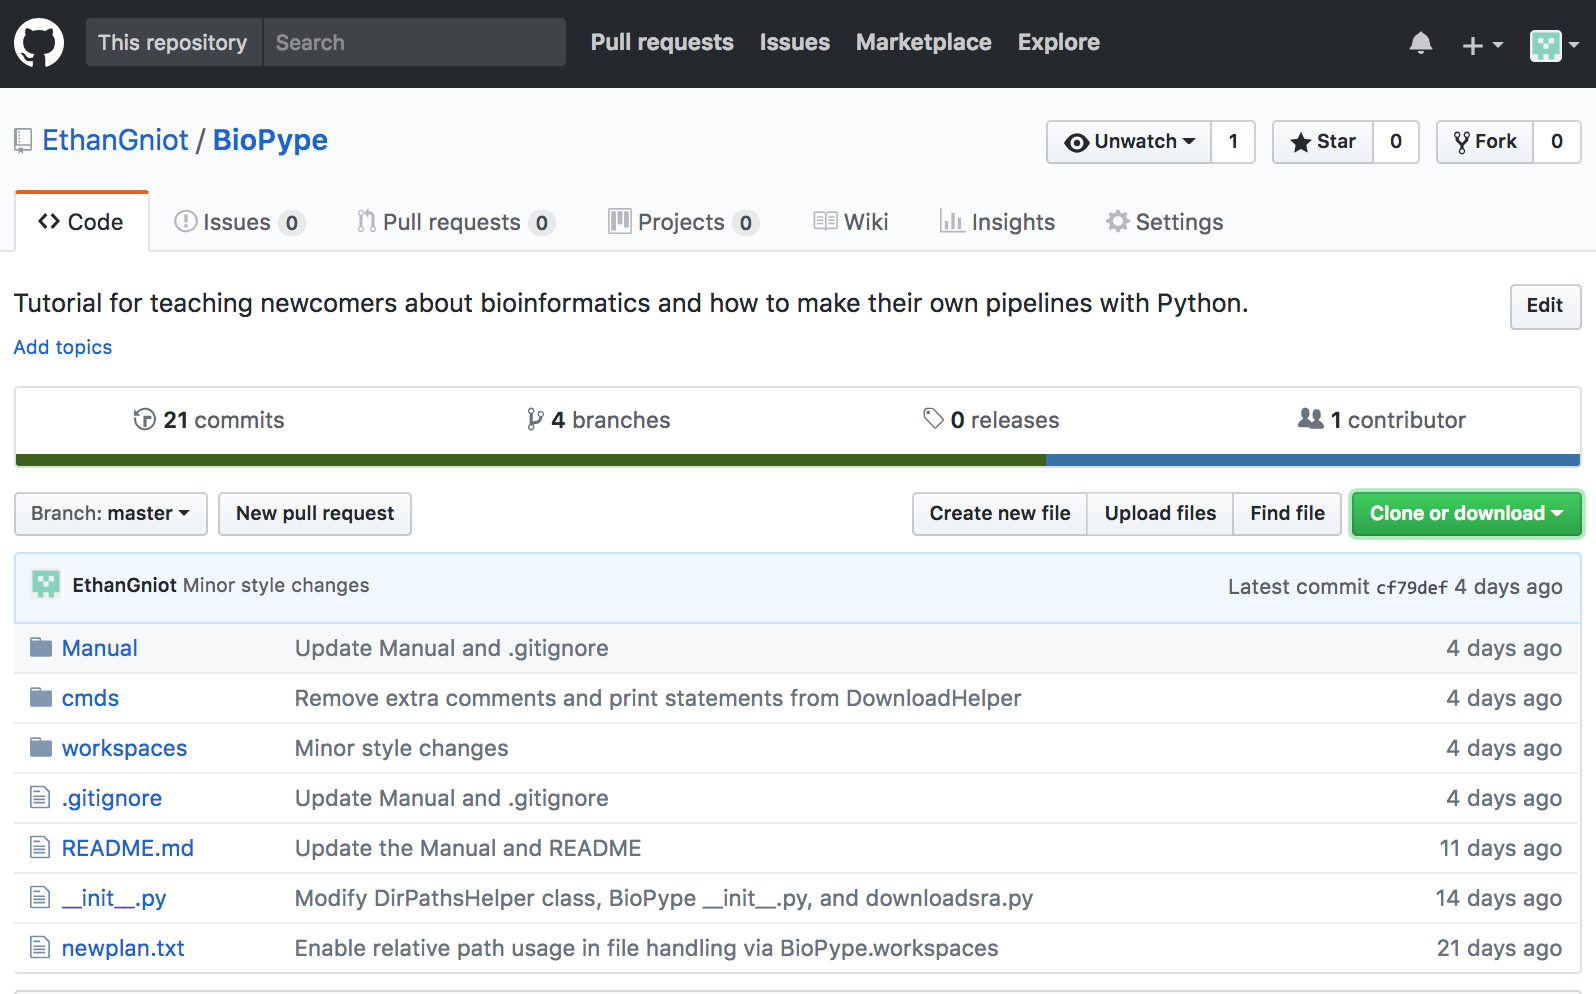
\includegraphics[height=8.5cm, width=13cm]{biopype-github}
    \caption{The BioPype Github webpage.}
    \label{fig:biopype-github}
    \hrule
    \end{maxipage}
\end{figure}


\item Click on the "biopype-dependencies.txt" file to view its contents. Next, right-click on the "Raw" button situated to the top-right of the text field and select "Save Link As...". Save the file to your Home folder (for most users, this should be the folder that shares your username). 


\item Open your computer's command-line application (on a Mac, this is the Terminal application). In the Terminal prompt, type the following and then press "Enter" (Note: the "\$" symbol represents the terminal prompt where you type. Do not actually type the \$):
    \begin{lstlisting} [basicstyle=\small, language=Python]
$ pwd
    \end{lstlisting}

The next line in the Terminal should then display a file path that represents your "current working directory". The current working directory is essentially the "folder" that your Terminal is currently looking at. It can see all the files and folders in that directory and access them by name if you ask it to. \seealso{For more information on navigating your files via the command-line, see Appendix \ref{appendix:command-line-navigate}. } For most users, this file path should lead to your home directory (e.g., /Users/your-username ). If the file path does not lead to your home directory, please read Appendix \ref{appendix:command-line-navigate} to learn how to change your current working directory to your home directory. 

\item Enter the following command in the Terminal prompt and then press "Enter":
    \begin{lstlisting} [basicstyle=\small, language=Python]
$ ls
    \end{lstlisting}

The Terminal should now display a list of all the files and folders in your current working directory. If you can't see the "biopype-dependencies.txt" file in the list, double-check that you downloaded it to your home directory. If you can see the file in the list, proceed to the next step.


\item To install all of the dependencies needed to run BioPype, enter the following into the command prompt:
    \begin{lstlisting} [basicstyle=\footnotesize, language=awk]
$ conda create --name biopype --file biopype-dependencies.txt
    \end{lstlisting}
The Terminal will take a while to think after you press "Enter" as it prepares to download all of the necessary packages. The different parts of this command accomplished several things:
    \begin{enumerate}
        \item \verb|conda|: this tells the Terminal that we want to execute one of conda's functions.
        \item \verb|create|: the conda function we want to use is the "create" function, which creates a new conda \textbf{virtual environment}. \seealso{For information on \textbf{virtual environments}, what they are, and why they're useful, see Appendix \ref{appendix:virtual-environments}.}
        \item \verb|--name|: this tells the Terminal that we are about to tell it what to name the new virtual environment.
        \item \verb|biopype|: this is the name of the new virtual environment.
        \item \verb|--file|: this tells the Terminal that we are about to tell it the name of a file containing dependencies that we want it to use when creating the new environment.
        \item \verb|biopype-dependencies.txt|: this is the name of the file containing the dependencies.
    \end{enumerate}
    After the terminal finishes thinking you will see the normal empty command prompt again. You should now have all of BioPype's dependencies installed in the "biopype" virtual environment. 


\end{enumerate}


\subsection{Installing dependencies with Anaconda}
This method is longer than the Miniconda method, so it will be broken up into three sections: 1) Installing and opening Anaconda, 2) creating a new virtual environment, and 3) installing dependencies.

\subsection*{Installing and Opening Anaconda}

\begin{enumerate}
    \item Go to the download page for the Anaconda distribution at \\ \url{https://www.anaconda.com/download}. 
    \item Select your preferred operating system from the Windows, macOS, or Linux tabs, then select the Download option for the \textbf{Python 3.6 version} (Figure \ref{anaconda_download}) and follow the installation instructions.

\begin{figure}[hbtp]
    \begin{maxipage}
    \hrule
    \centering
    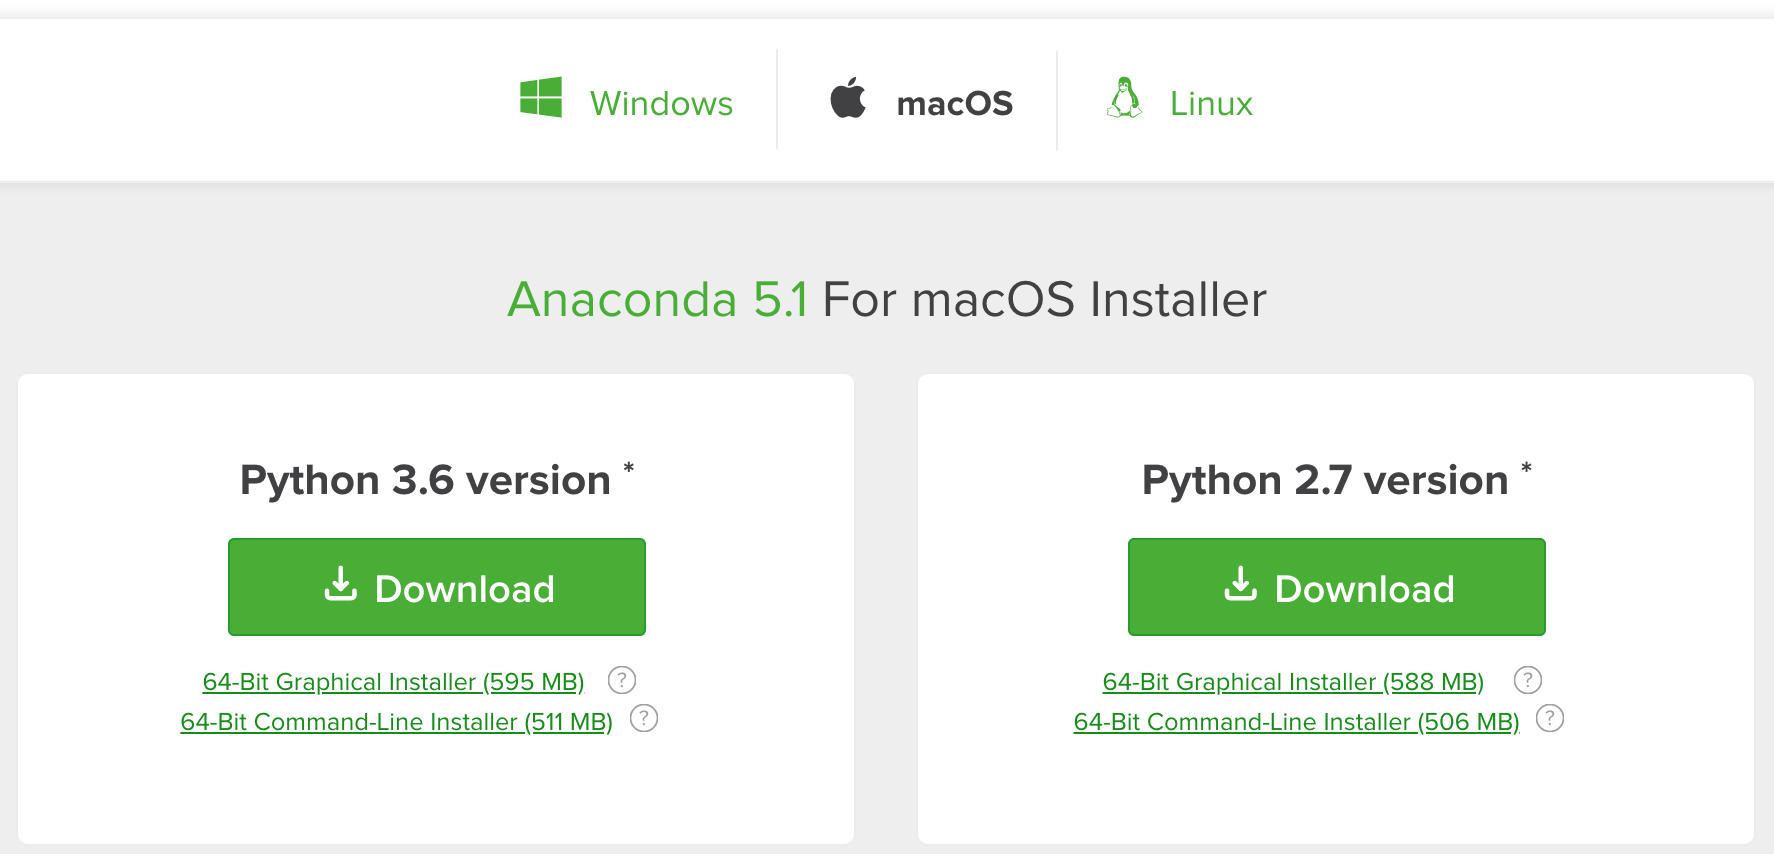
\includegraphics[height=5cm, width=9.5cm]{anaconda_download}
    \caption{The Anaconda download options provided on the Anaconda distribution website at \protect \url{https://www.anaconda.com/download}.}
    \label{anaconda_download}
    \hrule
    \end{maxipage}
\end{figure}


    \item After installation is complete, open the application named "Anaconda-Navigator" (the icon looks like 
\includegraphics[width=0.5cm]{anaconda-navigator-thumbnail}). After a brief start-up period, you should see the following window (Figure \ref{anaconda-nav-win}):
    
\begin{figure}[hbtp]
    \begin{maxipage}
    \hrule
    \centering
    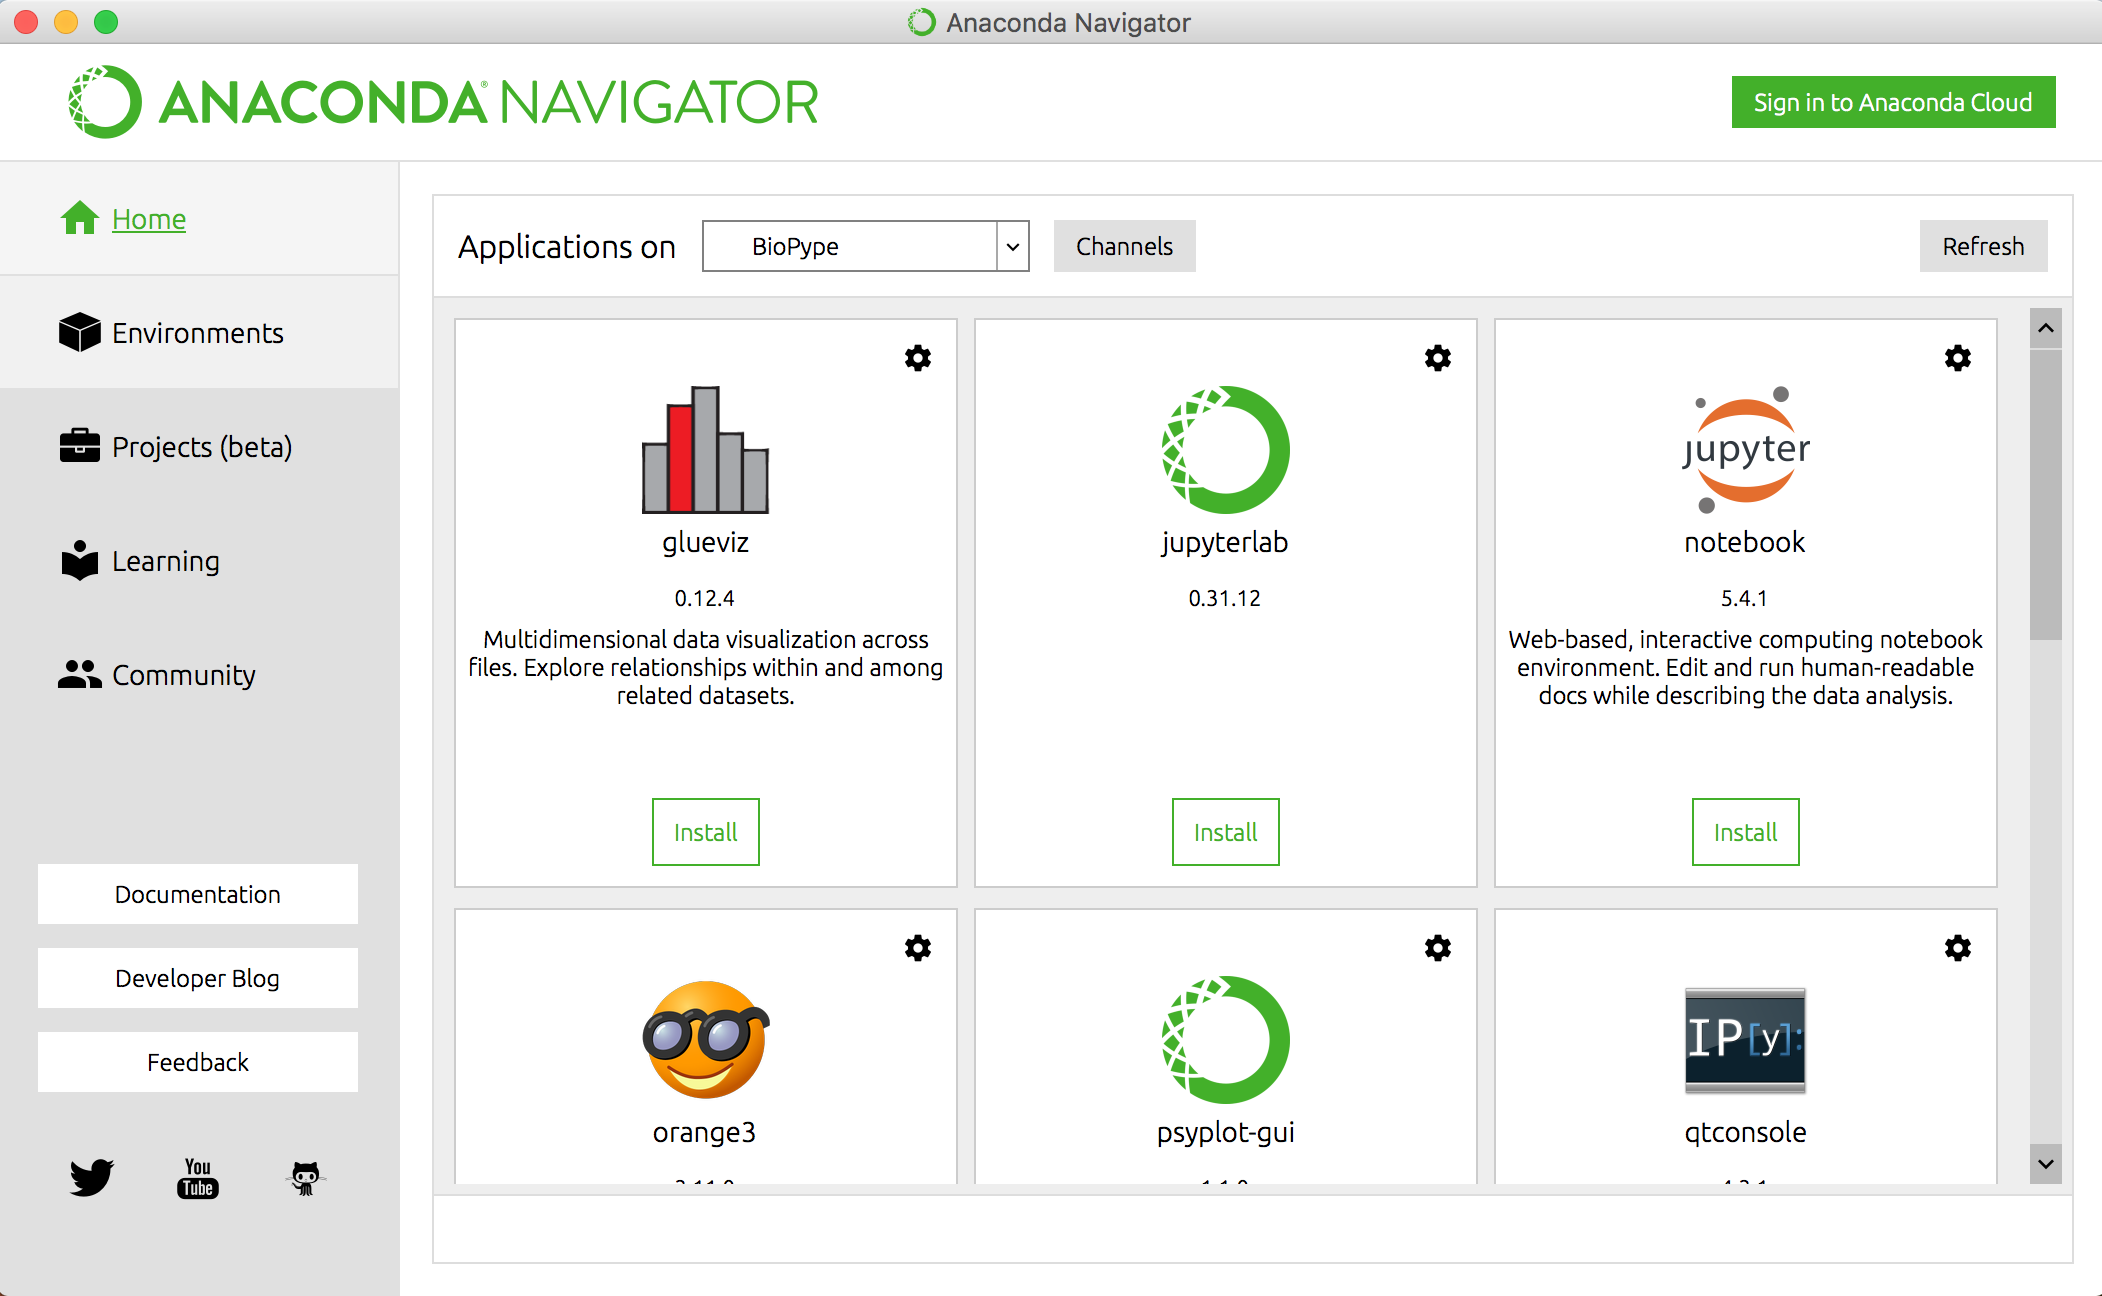
\includegraphics[height=7cm, width=11cm]{anaconda-nav-win}
    \caption{The window displayed to the user upon opening Anaconda-Navigator.}
    \label{anaconda-nav-win}
    \hrule
    \end{maxipage}
\end{figure}
    
    
\end{enumerate}

\subsection*{Create a New Virtual Environment}
    \todo[inline]{Link to resource for further reading on virtual environments}
    
    \begin{enumerate}
        \item \marginlabel{Make sure the computer has an internet connection while completing this section, otherwise Anaconda will not let you create a virtual environment.} On the left side of the Anaconda-Navigator window, click on the tab labeled \textbf{Environments}. (Figure \ref{anaconda-env-win}) 
        
\begin{figure}[hbtp]
    \begin{maxipage}
    \hrule
    \centering
    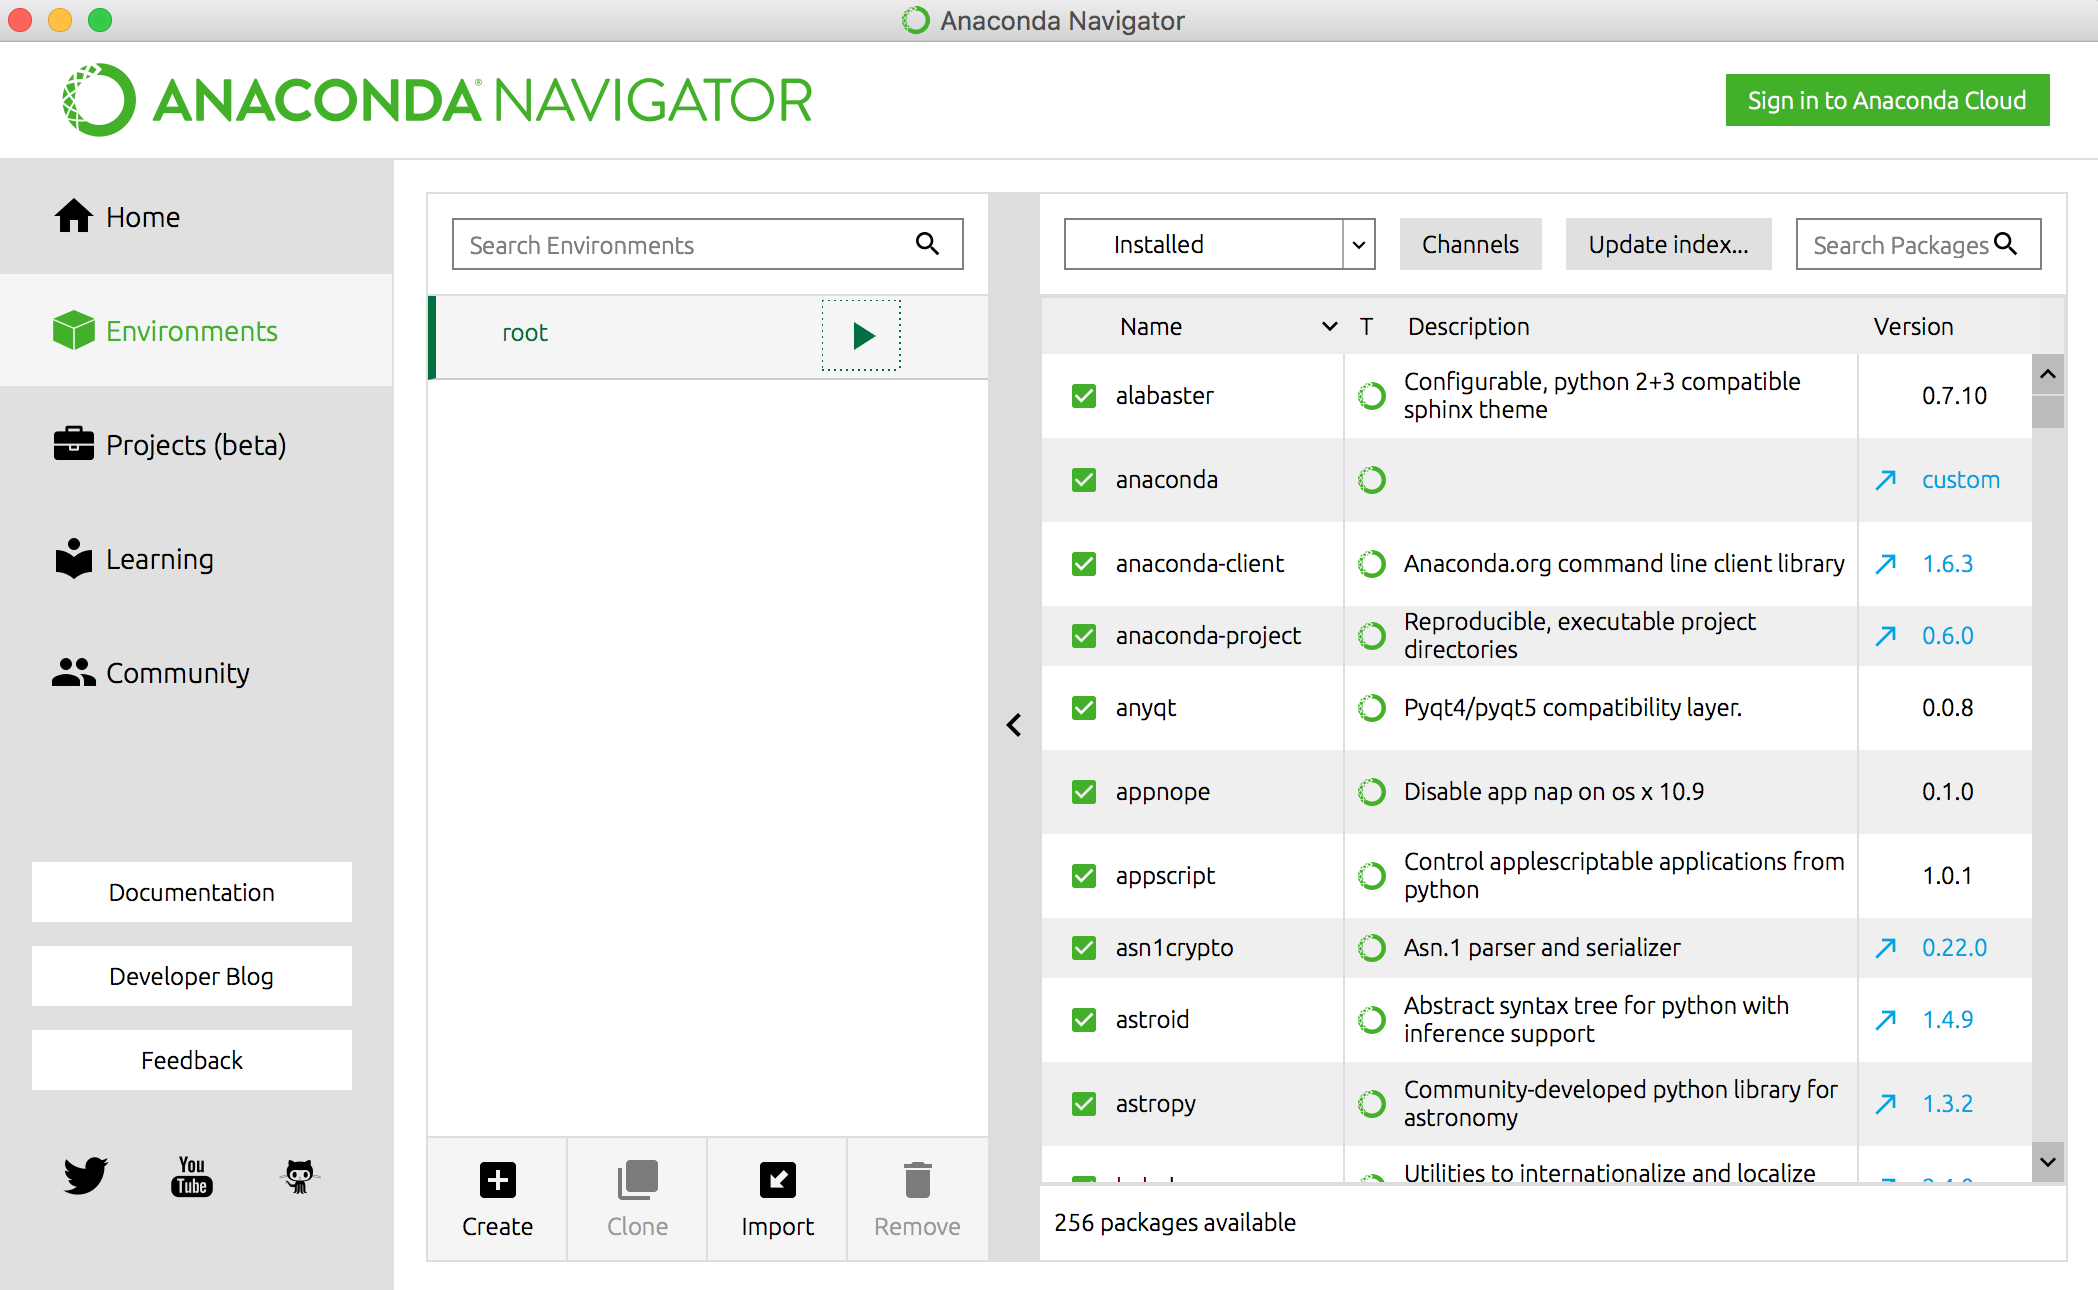
\includegraphics[width=12cm]{anaconda-env-win}
    \caption{The Environments window of the Anaconda-Navigator.}
    \label{anaconda-env-win}
    \hrule
    \end{maxipage}
\end{figure}
        \item Click the \textbf{Create} button on the bottom of the center panel. A new window titled "Create new environment" will appear. (Figure \ref{anaconda-create-new-env-win})

\begin{figure}[hbtp]
    \begin{maxipage}
    \hrule
    \centering
    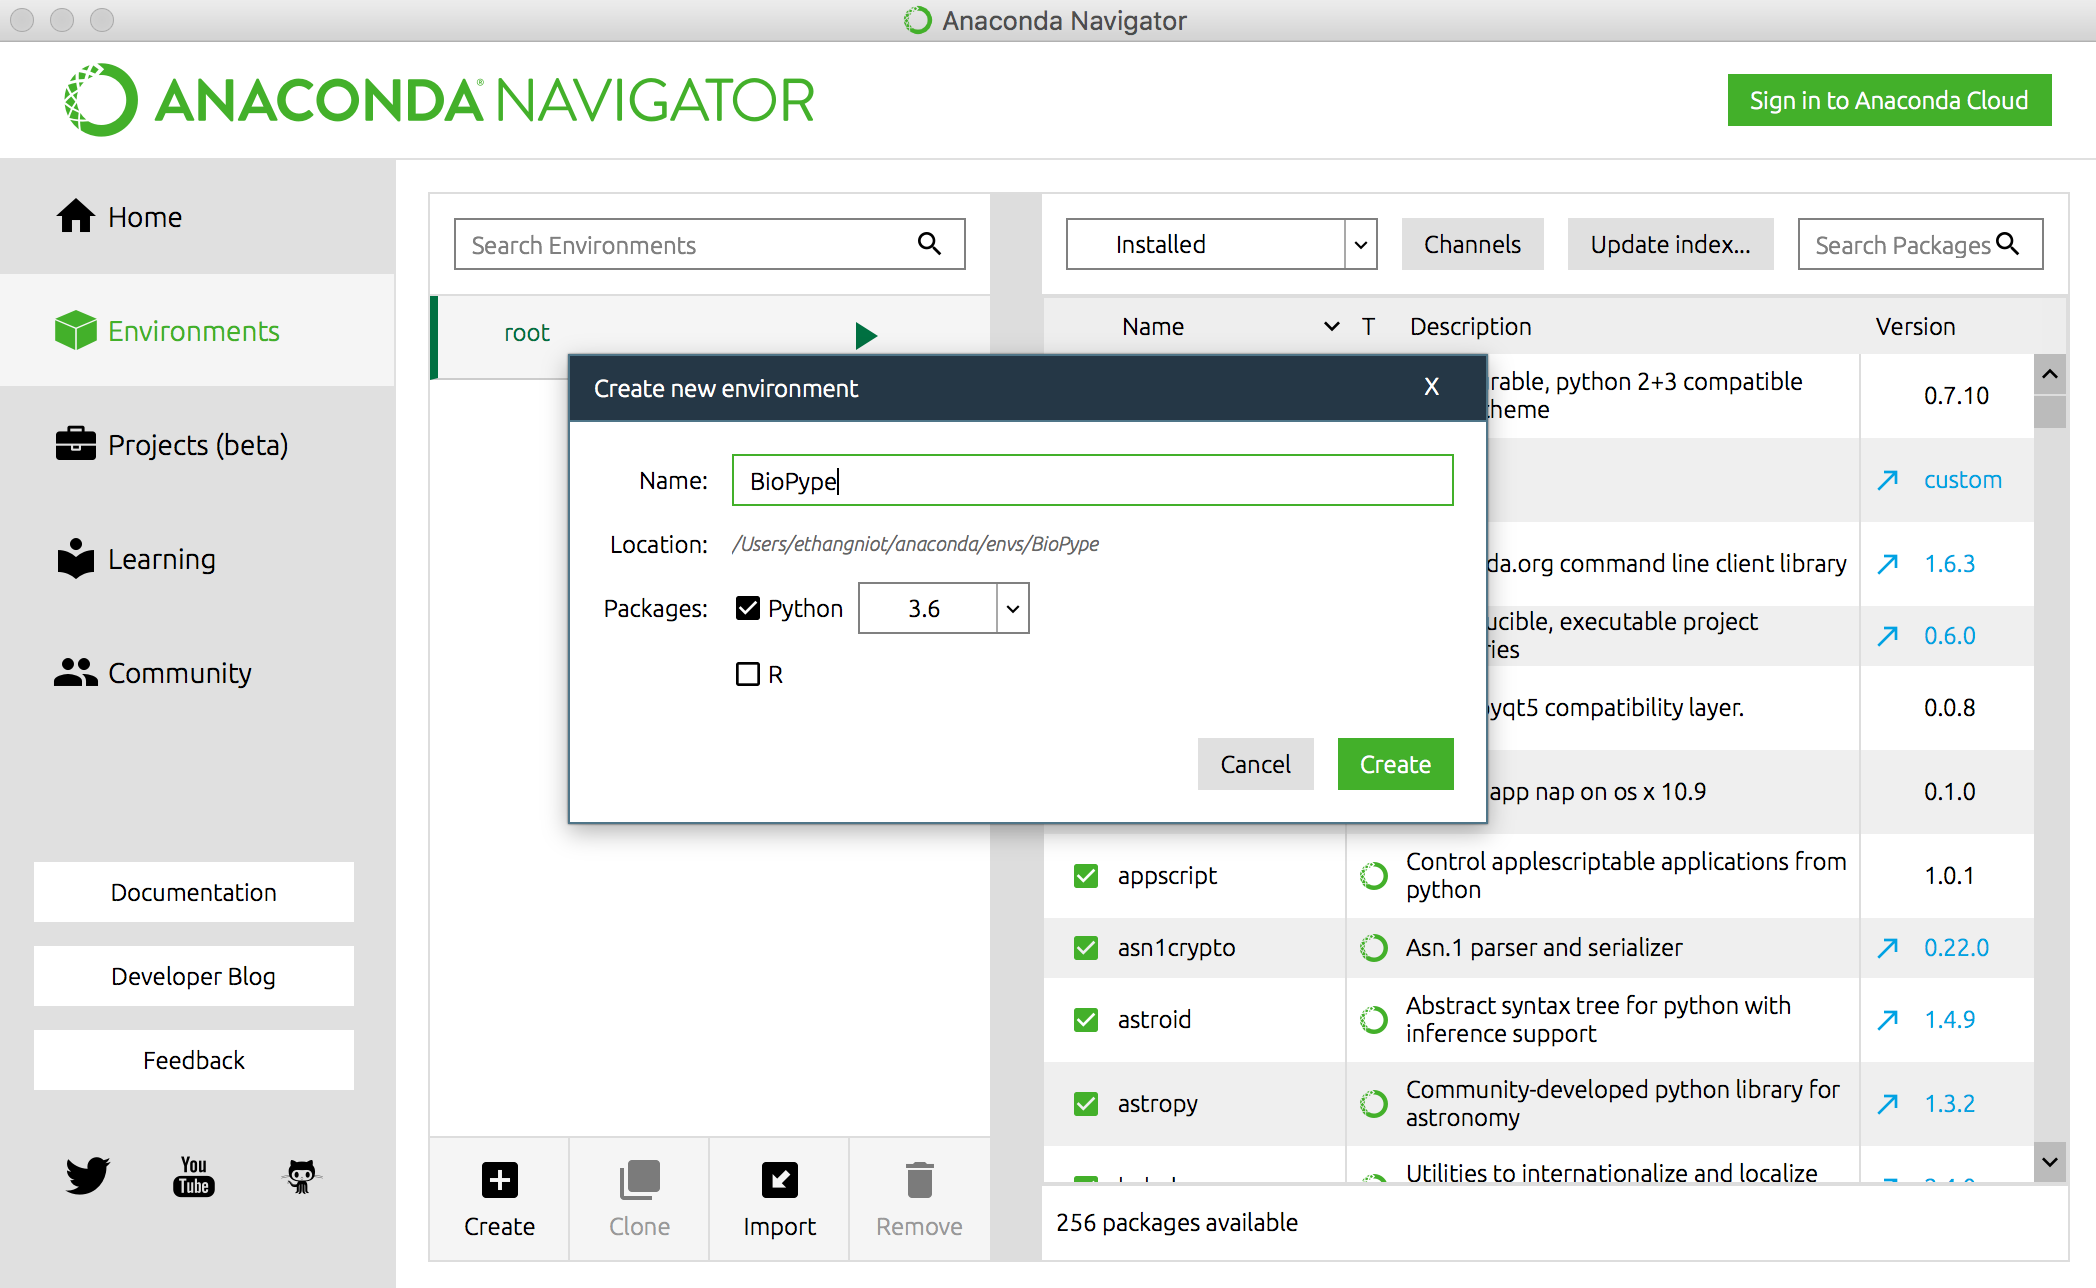
\includegraphics[width=12cm]{anaconda-create_new_env_win}
    \caption{The "Create new environment" window.}
    \label{anaconda-create-new-env-win}
    \hrule
    \end{maxipage}
\end{figure}
        
        \item Enter a \textbf{Name} for the environment. You may choose any name you want, but for the sake of this tutorial we will name the new environment "biopype".
        \item Select the box labeled \textbf{Python} next to the \textbf{Packages} heading.
        \item Choose a version of Python from the adjacent drop-down menu (Python 3.6 is the most current version at the time of this writing, but the packages we use require Python 3.5 so we chose \textbf{3.5}. If you are following the tutorial analysis in this manual, choose version 3.5).
        \item Click the \textbf{Create} button within the "Create new environment window".
    \end{enumerate}

\subsection*{Install packages}
    \begin{enumerate}
        \item Change Anaconda's current environment from the \textbf{root} environment by selecting the \textbf{biopype} tab in the middle panel of the Environments window.
        \item Click on the drop-down menu in the right-hand panel that says "Installed" and change it to "All".
        \item In the "Search Packages" box we can search for the packages that BioPype needs in order to function. For instance, if BioPype depended on the "biopython" package, we could enter "biopython" into the box. The search should then return a package named "biopython". We would then select the checkbox to the left of the name. (Figure \ref{anaconda-search-pack})
        \begin{itemize}
            \item A pair of green and red boxes (reading "Apply" and "Clear", respectively) will appear in the bottom-right of the window once a package is selected. Do not click these just yet. 
    %

\begin{figure}[hbtp]
    \begin{maxipage}
    \hrule
    \centering
    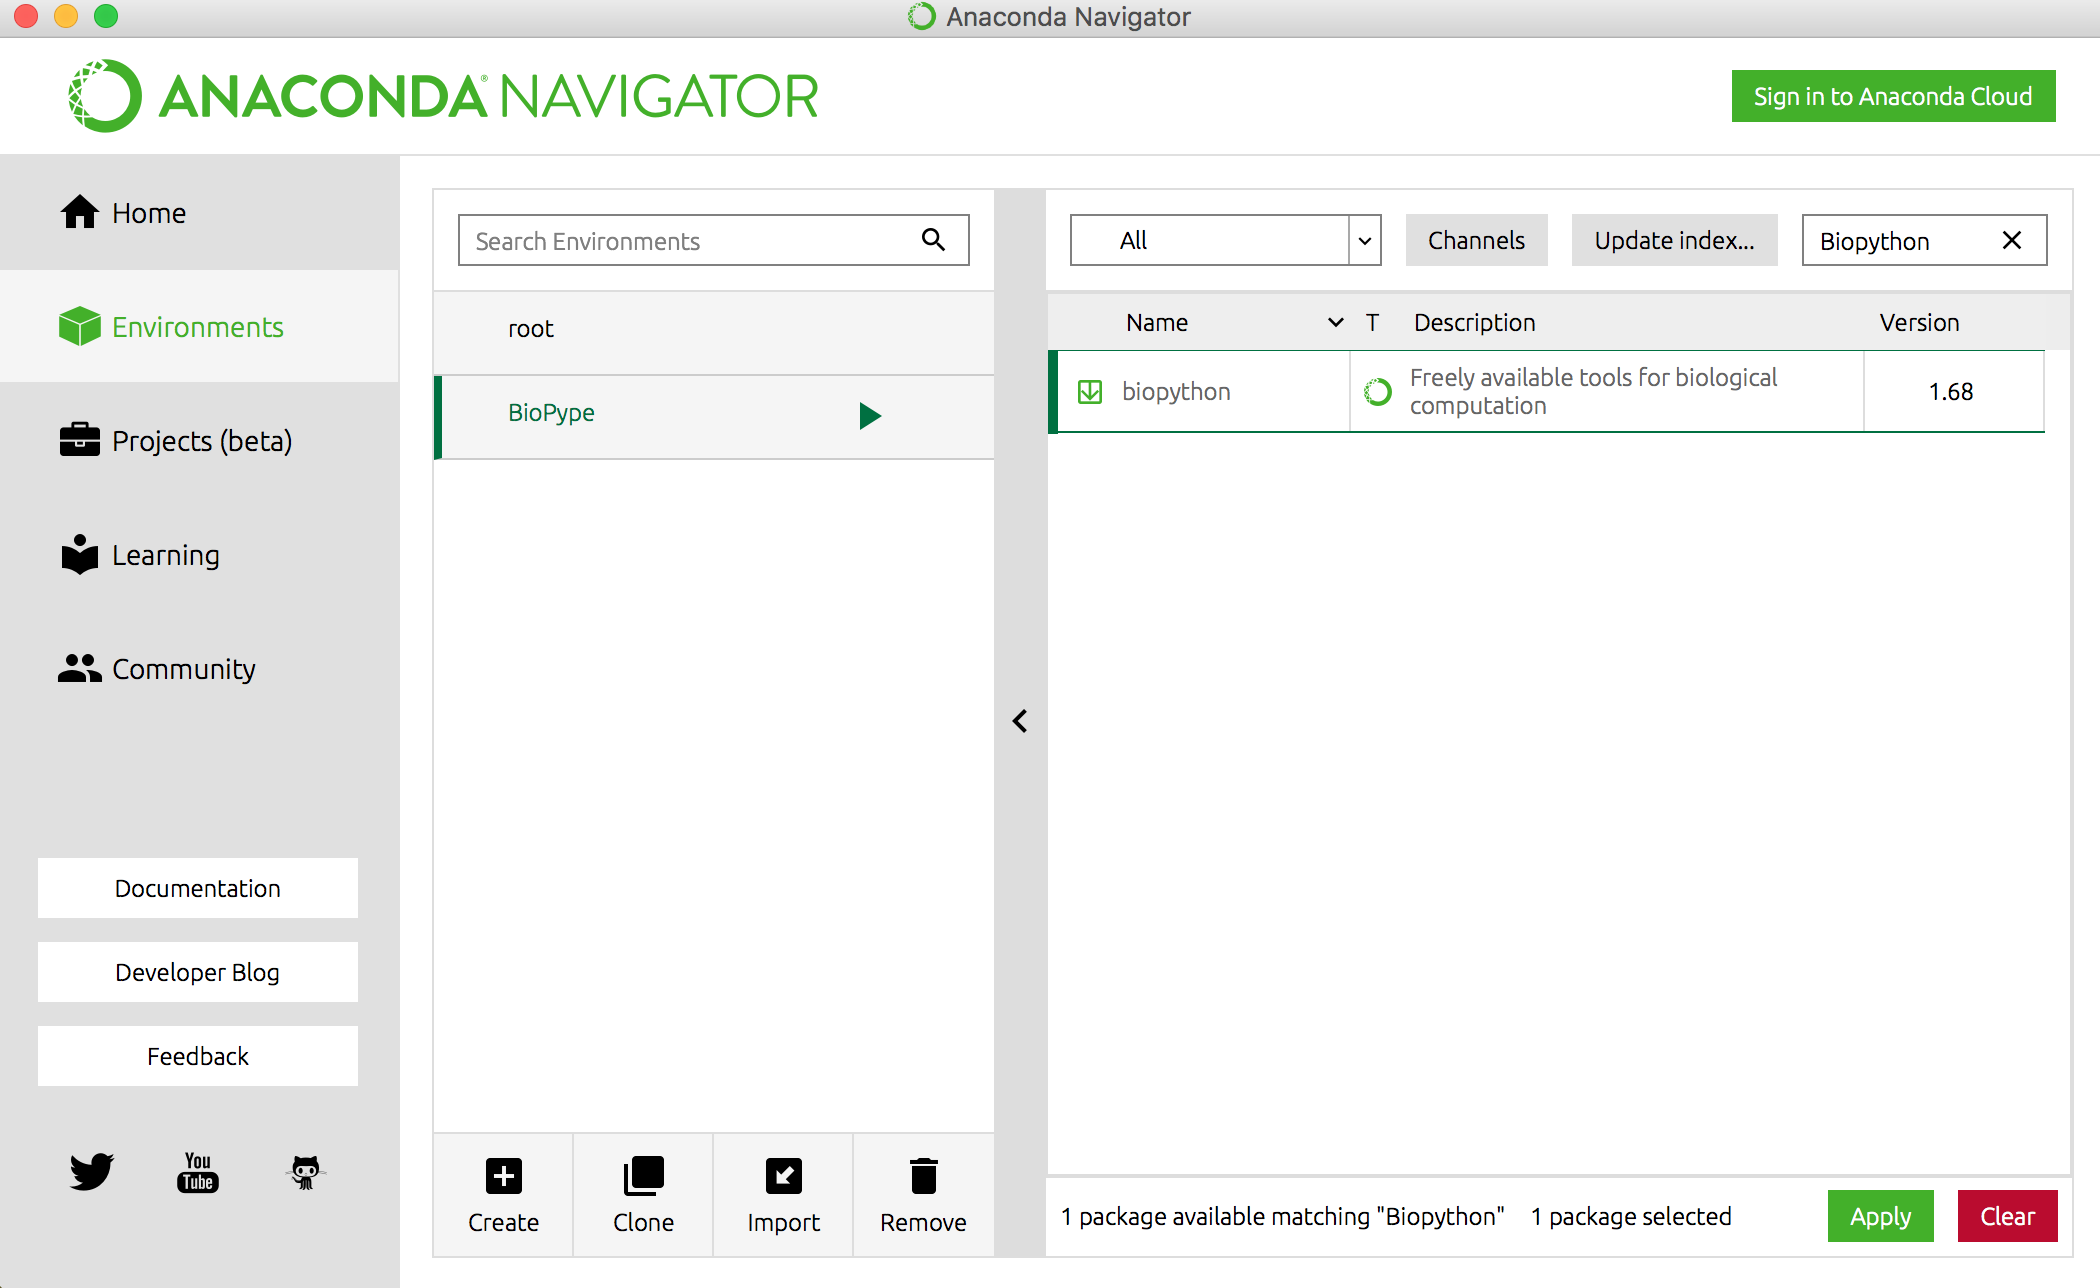
\includegraphics[width=12cm]{anaconda-search-pack}
    \caption{Searching for a package. When a package is selected, the checkbox next to the package's name will be green.}
    \label{anaconda-search-pack}
    \hrule
    \end{maxipage}
\end{figure}
    %
        \end{itemize}
        \item Use the search bar to find and select the packages listed in \autoref{tab:software} (except qiime2. That will need to be added to the environment by obtaining the .yml file from the qiime2 installation link and using the \verb|conda env install --name <env-name> --file qiime2-2018.4-py35-osx-conda.yml| command). Once all packages have been selected, click the green "Apply" button in the bottom right corner of the window, then select "Apply" again within the "Install Packages" window that appears. (Figure \ref{anaconda-install-pack}) Anaconda will now install the selected packages.
        \begin{itemize}
        \item Note: it may take a while for the windows to fully load when selecting "Apply" and "Install Packages", due to so many being selected at a time. 
        \end{itemize}
    %

\begin{figure}[hbtp]
    \begin{maxipage}
    \hrule
    \centering
    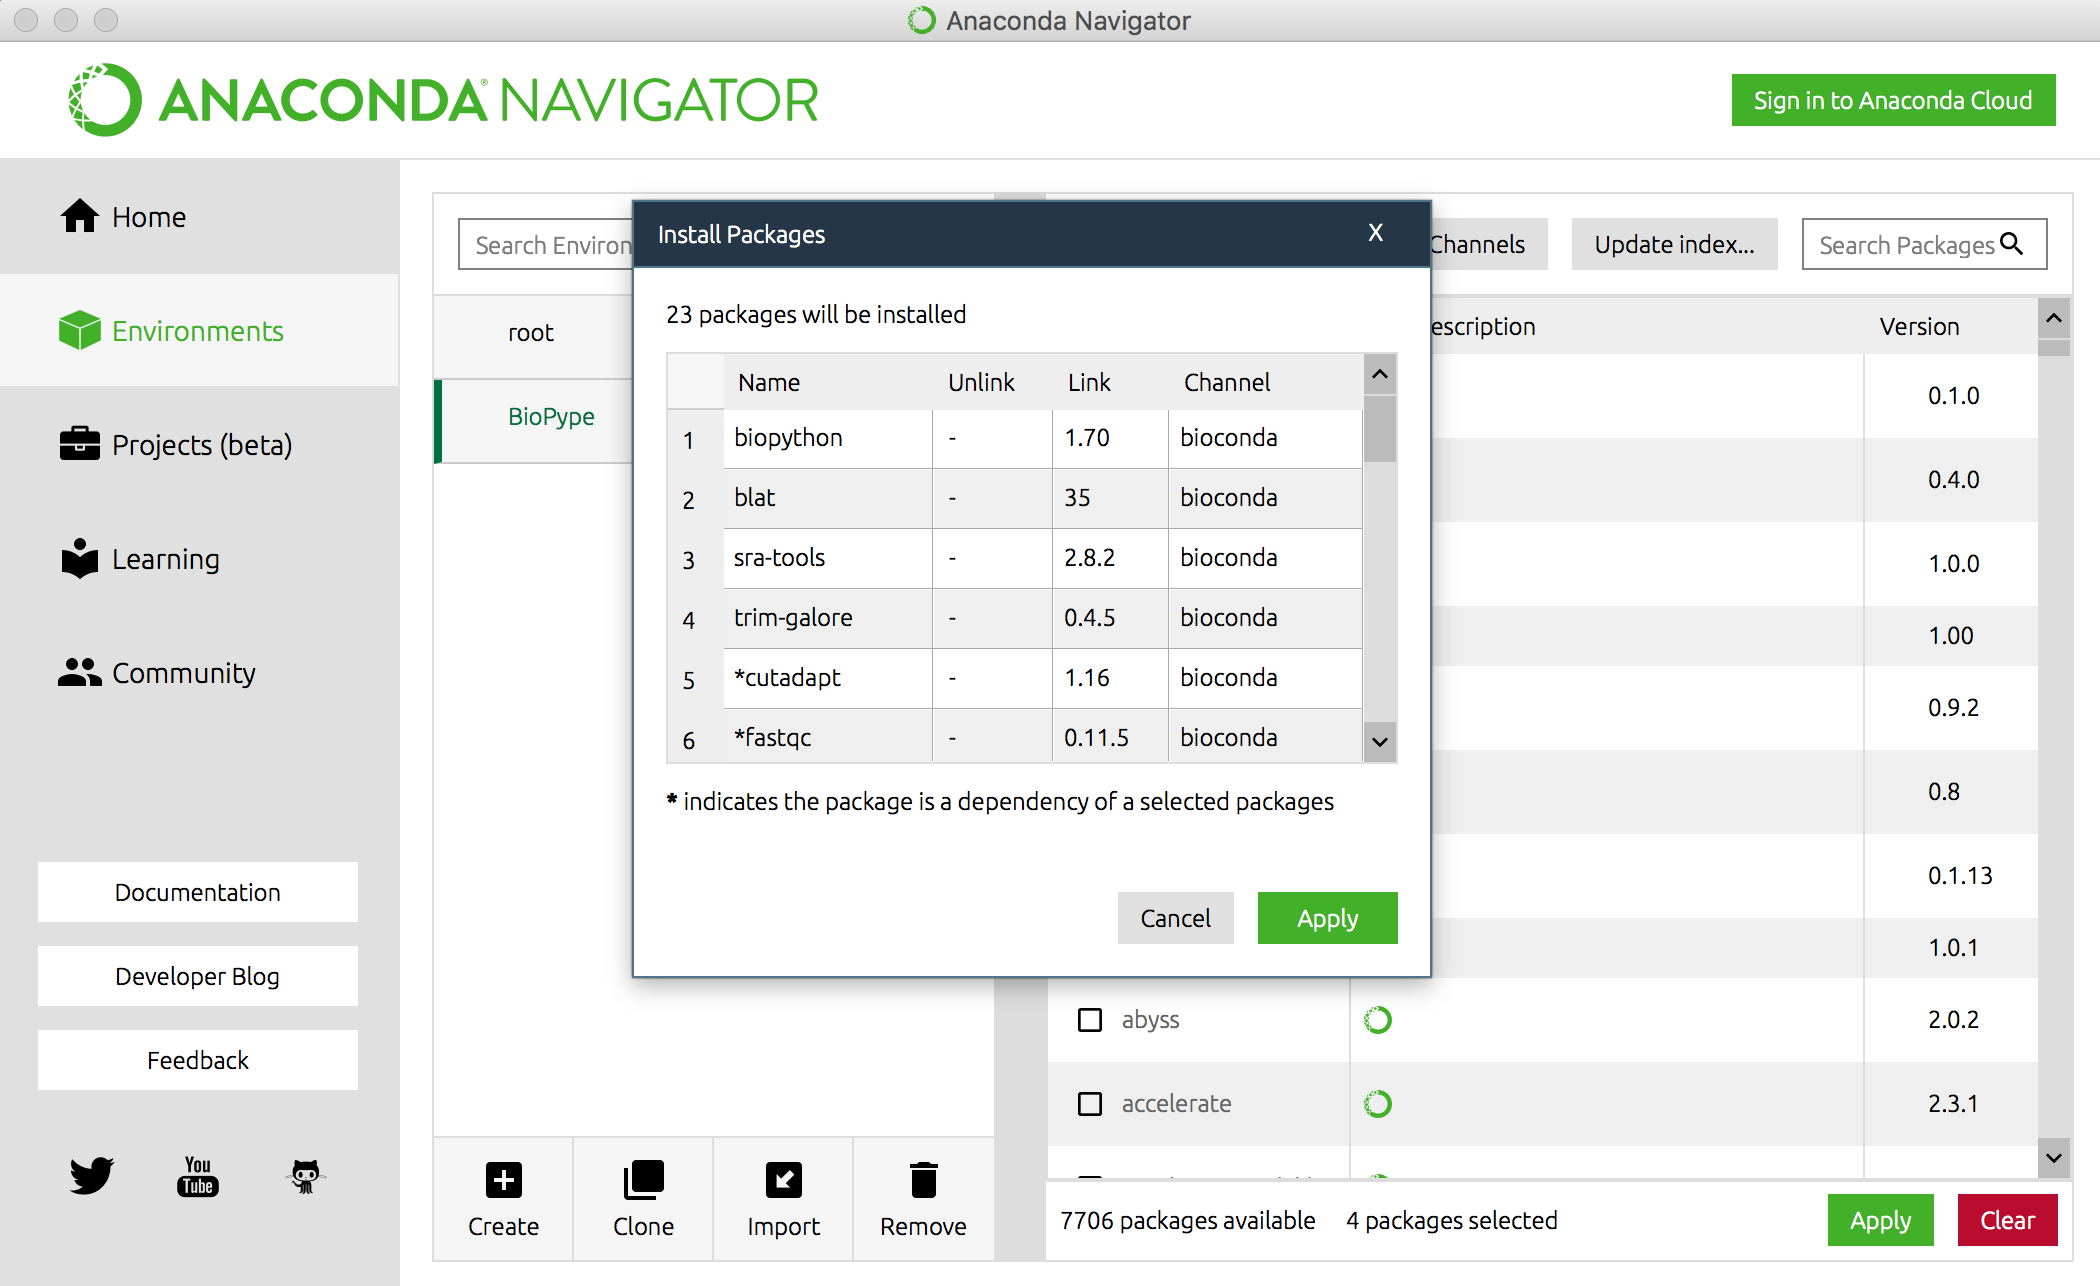
\includegraphics[width=12cm]{anaconda-install-pack}
    \caption{The window displaying the packages and dependencies that will be installed.}
    \label{anaconda-install-pack}
    \hrule
    \end{maxipage}
\end{figure}
    
    \end{enumerate}


\subsection{Downloading BioPype}

With the dependencies installed, we now need to download BioPype. 

\begin{enumerate}
\item Go back to the BioPype Github repository at \url{https://github.com/EthanGniot/BioPype}. (See Figure \ref{fig:biopype-github}).

\item Click on the green "Clone or download" button (see Figure \ref{fig:biopype-github})
    \begin{itemize}
    \item \small Note: The Github page that the URL from step 1 brings you to contains the code for the most recent "master" update to the BioPype repository. The "master" updates are usually the most recent \textit{stable} versions of BioPype. However, there may also be other versions of BioPype that are newer, but may contain bugs due to being under active development. To access these versions, click on the "branches" link (in Figure \ref{fig:biopype-github}, it is the link that says "4 branches" next to a branching symbol). If there are any branches (i.e., "versions") of BioPype that are more-current than the "master" branch, you will be able to see them on this page. This page also has links to the branches, where you can download that version of the BioPype code.
    \end{itemize}
%
\item Click on the "Download ZIP" button (the blue button in Figure \ref{fig:biopype-download}).
    \begin{figure}[hbtp]
        \begin{maxipage}
        \hrule
        \centering
        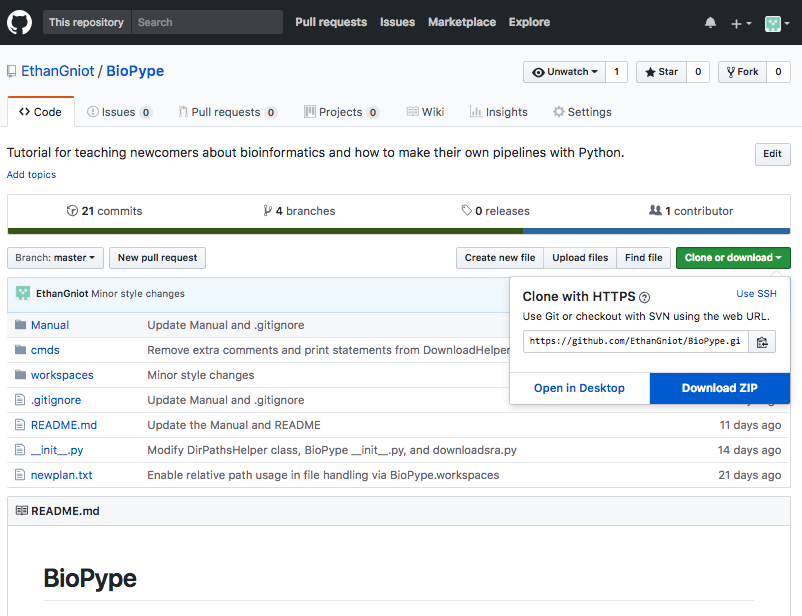
\includegraphics[height=8.5cm, width=13cm]{biopype-download}
        \caption{The button to download the BioPype code repository as a .zip file.}
        \label{fig:biopype-download}
        \hrule
        \end{maxipage}
    \end{figure}
    

\item Navigate to your Downloads folder and unzip the BioPype .zip file. 


\item Copy the BioPype folder, then navigate to the following file path and paste the folder into the "site-packages" folder (note: the parts of the file path that are in parentheses are not the literal names of directories. Substitute the appropriate directory into those spots based on the name of your home folder and whether you chose Anaconda or Miniconda):\newline
(home-folder)/(Anaconda-or-Miniconda)/envs/biopype/lib/python3.5/site-packages

\end{enumerate}


%
\subsection{The BioPype Project Directory and the SRA Toolkit Workspace Location}
To perform a microbiome analysis with BioPype, we will need a location where we can save our data and files. 
\begin{enumerate}

\item \marginlabel{\small The \textbf{SRA database} is a place where researchers can upload the sequencing data they use in their experiments for public access. Along with the raw sequence data, they also provide information about the experimental methods they used in the study that the sequencing data come from. } Create a directory somewhere in your file system and name it \newline "biopype\_project". (Remember that microbiome sequencing files are very large, so make sure to create the project folder somewhere with a lot of free storage space.) 

One of the packages BioPype uses is the SRA Toolkit (the package name in your file system will be "sra-tools"). This package lets us download .sra files from the NCBI \textbf{Sequence Read Archive (SRA) database}. In order to use the package, it requires that a directory called the "Workspace Location" be configured first. 

\item Create a folder inside the \verb|biopype_project| directory called "data".
\item In the Terminal, navigate to the "bin" subdirectory of the sra-tools package using the \verb|cd <path-to-subdir>| Terminal command.
\begin{itemize}
\item The bin subdirectory will be \textit{very} deep in your file system. The following file path is where the subdirectory is located on my machine:\newline /Users/ethangniot/miniconda3/envs/biopype\_project/share/ncbi\\/sra-tools/mac/clang/x86\_64/rel/bin
\end{itemize}

\item In your web browser, go to \url{https://trace.ncbi.nlm.nih.gov/Traces/sra/sra.cgi?view=toolkit_doc&f=std#s-4} and follow the configuration instructions to change the Workspace Location to the "data" folder you created in the \verb|biopype_project| folder.

\item In the Terminal, navigate back to the biopype\_project folder.


\item Activate the "biopype" virtual environment by typing the following into the command prompt:
\begin{lstlisting} [language=awk]
$ source activate biopype
\end{lstlisting}

\item Activate the Python interpreter by typing the following into the command prompt:
\begin{lstlisting} [language=awk]
$ python3
\end{lstlisting}

\item Import BioPype into the current Python environment:
\begin{lstlisting} [language=python]
>>> import BioPype
\end{lstlisting}


\item Upon importing BioPype, you should see a prompt appear in the Terminal window telling you what the current working directory for BioPype is, as well as the current Workspace Location for the SRA Toolkit. To change the location of where BioPype thinks these directories are, enter the following command:
\begin{lstlisting} [language=python]
>>>BioPype.path_helper.setup('biopype')
\end{lstlisting}

\item The Terminal will now ask you to "input a path to an existing folder to define BioPype's working directory". Input the file path to the "biopype\_project" folder. (e.g., /Users/username/biopype\_project)

\item Once the previous command is finished running, execute the following:
\begin{lstlisting} [language=python]
>>>BioPype.path_helper.setup('sra')
\end{lstlisting}
A prompt should appear that asks you to "input the path for the SRA Toolkit's configured Workspace Location." Input the path to the "biopype\_project/data" directory that you configured as the Workspace Location in step 4 of this section.


\end{enumerate}
%

The BioPype package should now be fully configured and ready to use for microbiome analyses!

%



\chapter{The Dataset}
    %
    \begin{maxipage}
    \begin{bclogo}[couleur = vlightgray, logo = \bcinfo] {Recap}
    In the previous chapter, we set up our machine so that it has all of the software BioPype needs in order to function. \newline \newline In this chapter, we will use BioPype to \textbf{download} experimental data, and then prepare them for analysis via a process called \textbf{"quality control"}. We will also discuss how the BioPype functions used in this workflow were created.
    \end{bclogo}
    \end{maxipage}
    %

As described in Chapter \ref{chap:scene}, we want to investigate if there are any differences in the gut microbiomes of younger patients with IBD compared to older patients with IBD. Using the methods described in Chapter \ref{chap:find-tools}, we found a study in the SRA database with sequencing data that are useful to us. The webpage for the SRA Study is reproduced in Figure \ref{fig:ncbi-sra-study-page} and can be accessed at
    \url{https://trace.ncbi.nlm.nih.gov/Traces/sra/?study=SRP115494} .
    
%
\begin{figure}[hbtp]
    \begin{maxipage}
    \hrule
    \centering
    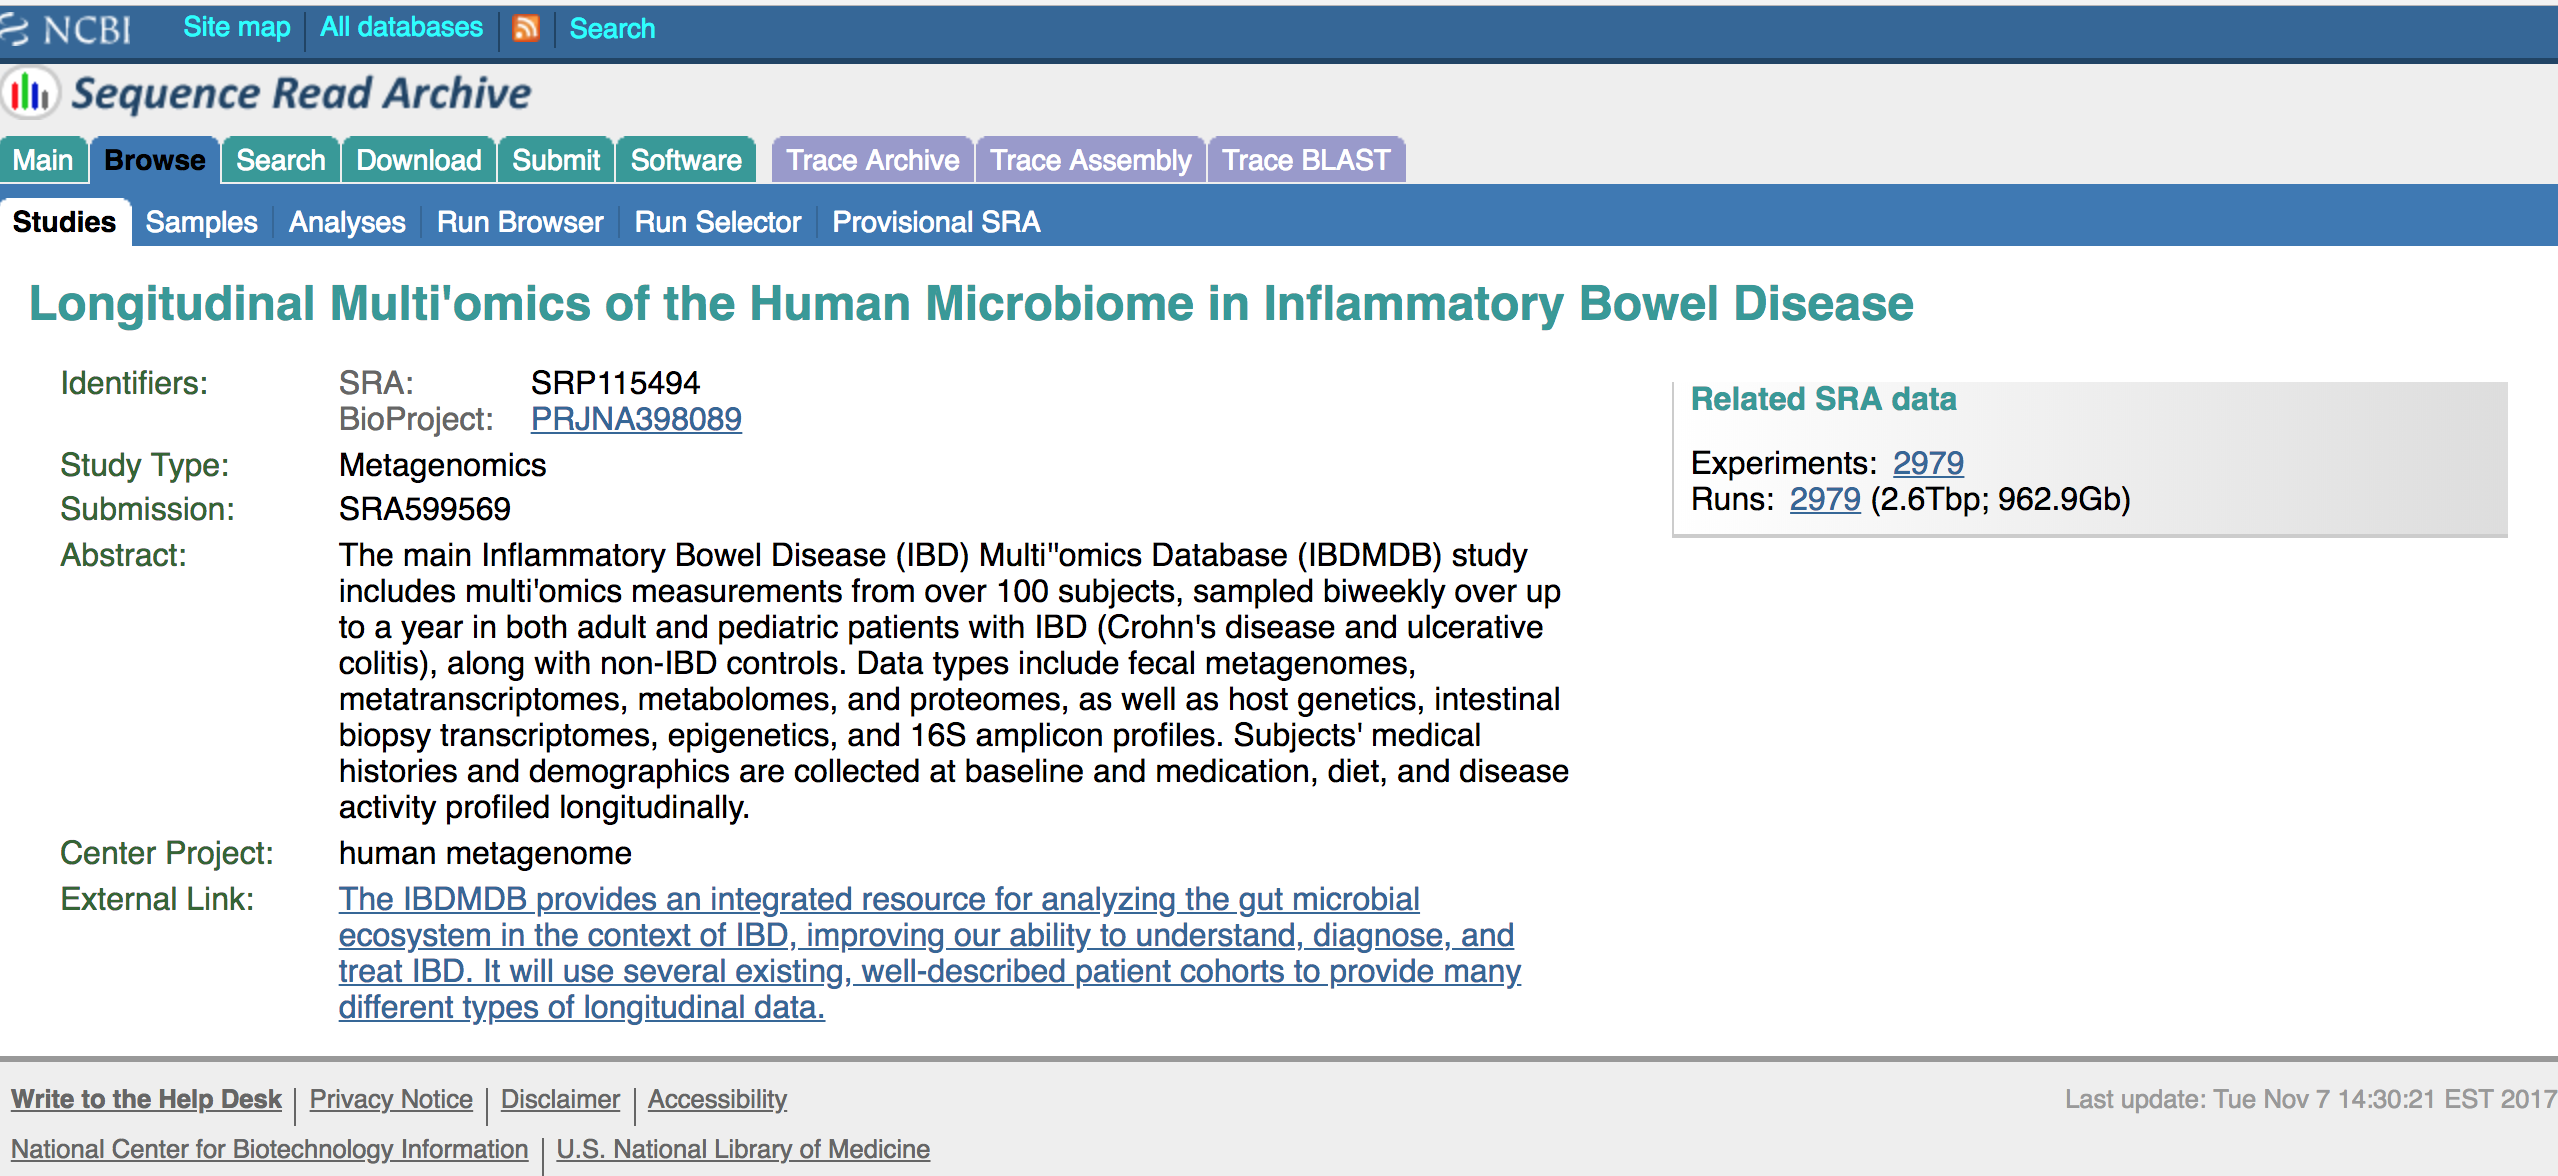
\includegraphics[height=8.75cm, width=16cm]{ncbi-sra-study-page}
    \caption{The "SRA Study" webpage.}
    \label{fig:ncbi-sra-study-page}
    \hrule
    \end{maxipage}
\end{figure}
%

The dataset is reproduced in Figure \ref{fig:ncbi-sra-runs-page} and can be found by clicking on "Runs" under "Related SRA data" on the right side of the SRA Study webpage, or by going to \url{https://trace.ncbi.nlm.nih.gov/Traces/study/?acc=SRP115494#} .

%
\begin{figure}[hbtp]
    \begin{maxipage}
    %\begin{center}
    \centering
    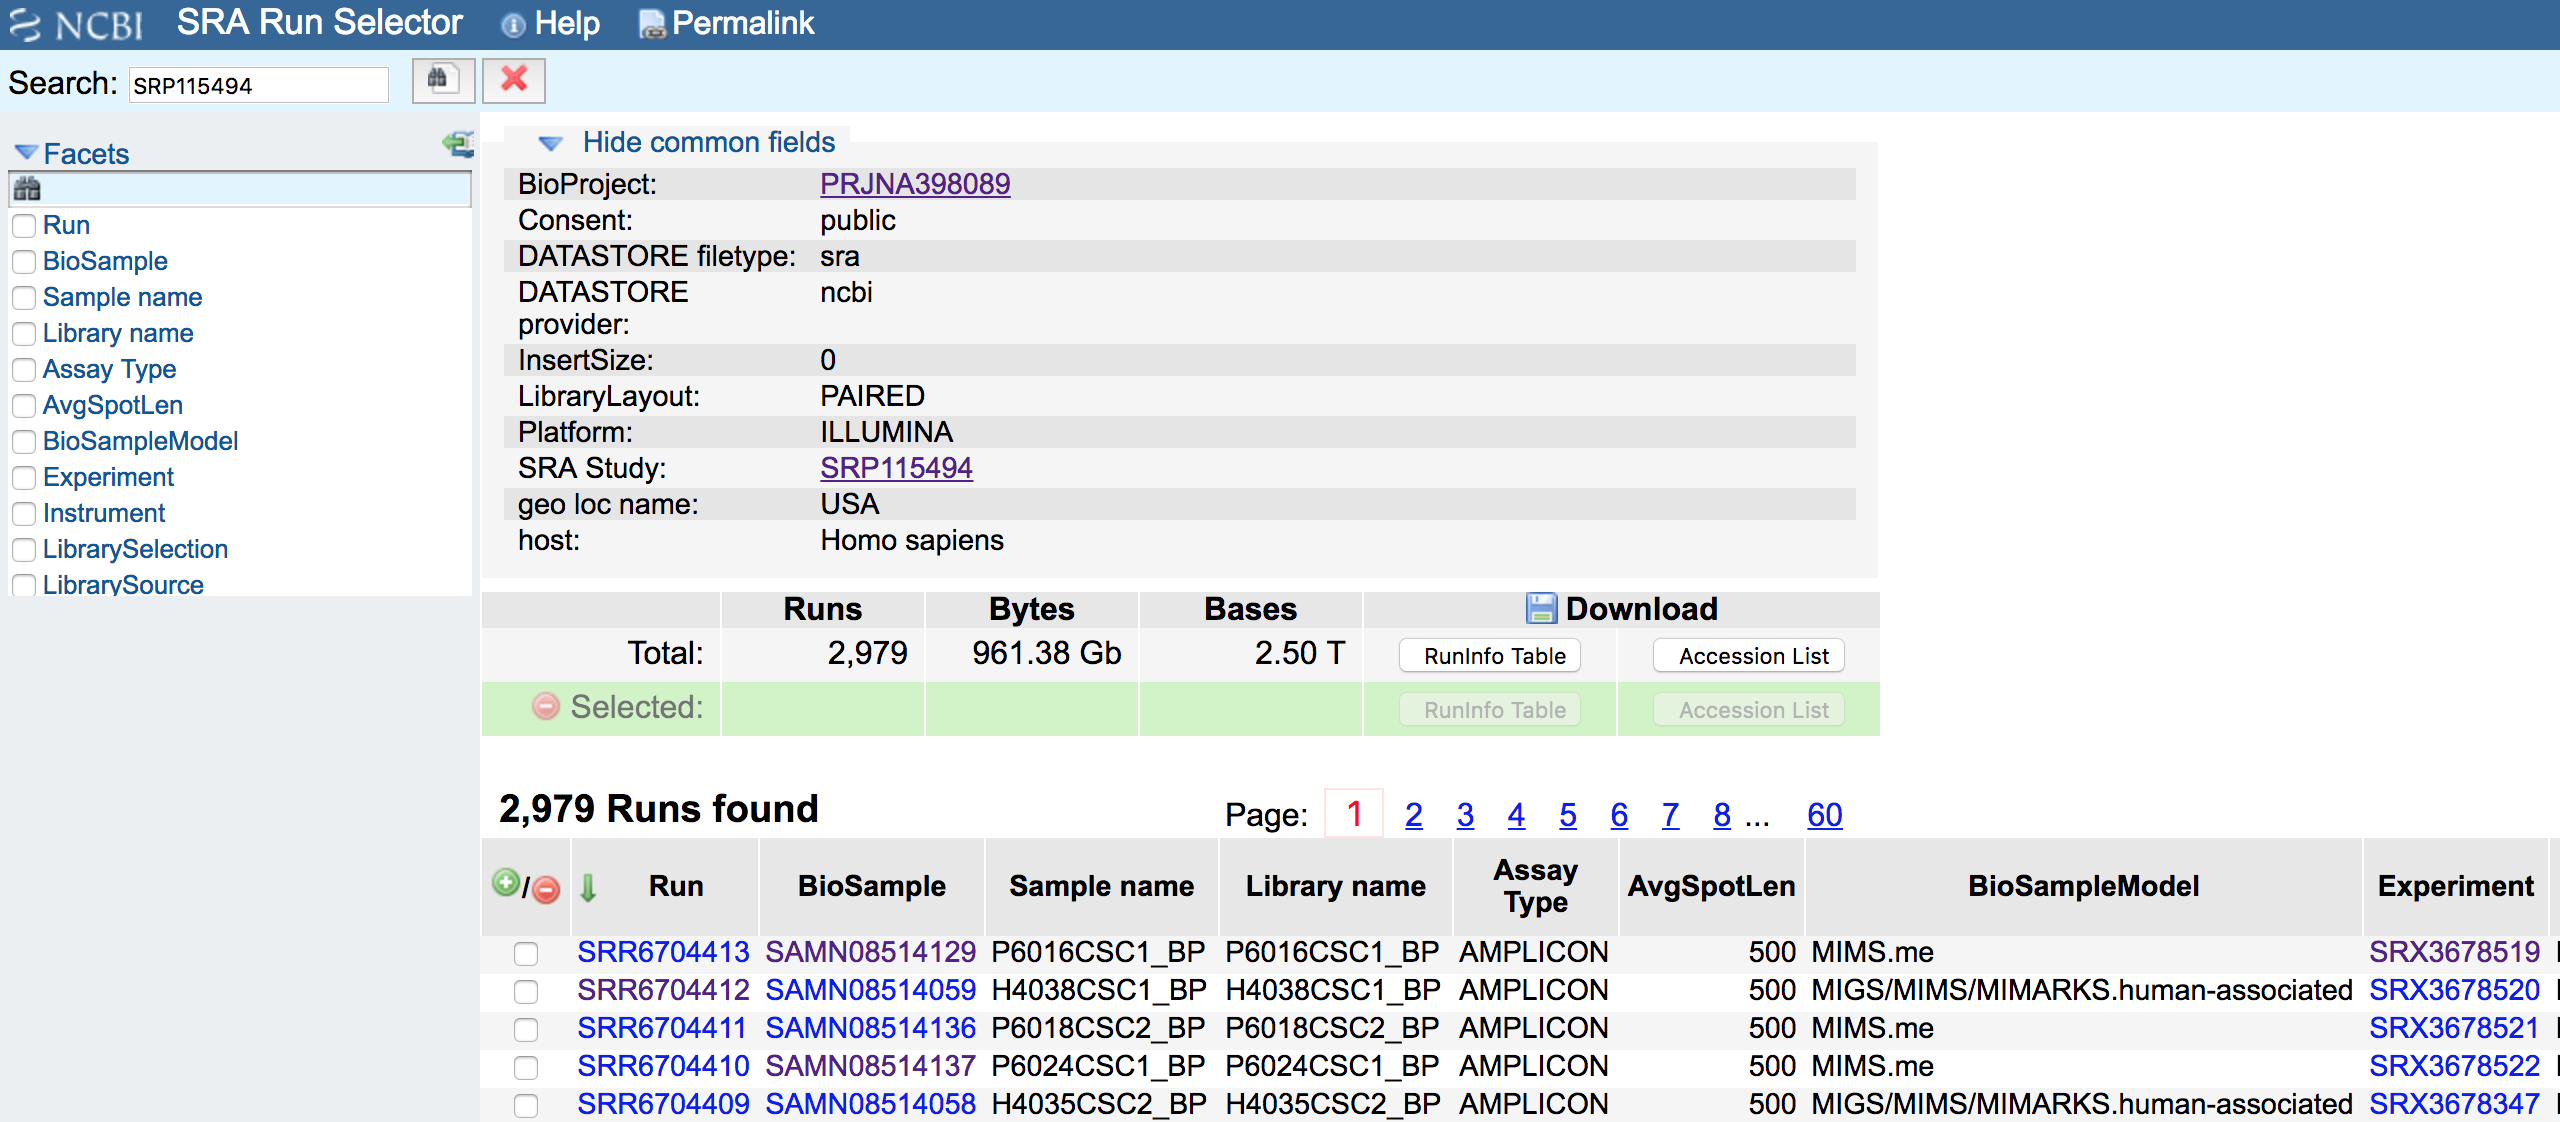
\includegraphics[height=8.5cm, width=16cm]{ncbi-sra-runs-page}
    \caption{The sequencing data collected by the \textit{Longitudinal Multi'omics of the Human Microbiome in Inflammatory Bowel Disease} study. (Note: the table's columns extend beyond the right side of the page because there are 36 metadata categories.)}
    \label{fig:ncbi-sra-runs-page}
    %\end{center}
    \end{maxipage}
\end{figure}
%
    
To learn more about how to use these pages to find information about the study and its methods, please refer to Chapter \ref{chap:find-tools}. 
    
    %
    \section{Download and Quality Control Dataset}
    
        \begin{enumerate}
            \item First, we must decide what criteria we will use to choose our experimental samples. 
            \marginlabel{Note: The dataset has a metadata category called "BioSample." This is not to be confused with the generic term "samples." In this case, one sample is equivalent to one run (i.e., one row) of the data table.}
            \newline
            Remember: our research question investigates the effects of age on the gut microbiomes of inflammatory bowel disease patients. Looking at the study abstract from Figure \ref{fig:ncbi-sra-study-page}, we can see that the researchers investigated two types of IBD: Crohn's disease and ulcerative colitis. So one of the metadata categories from the dataset (i.e., the columns from the dataset in Figure \ref{fig:ncbi-sra-runs-page}) that we will use to select our samples is the "host\_disease" category. We will also select our samples based on the "host\_age" metadata. Finally, our relative abundance analysis will require amplicon sequencing data, so the third metadata category we will sort by is the "Assay\_Type" column.
            
            \item Now we want to select our samples based on these categories. 
            
            Download the RunInfo Table file found on the study's sample page and put it in the project folder you set up in Chapter \ref{software}. The RunInfo table is just the browser's sample table in a .txt file format.
            
            \item Open the command line interface for your machine's operating system. On a mac, this is the Terminal application. 
            
            \item Navigate to your project's folder and then confirm that you are in the right location by using the the following commands at the command prompt:
            
                \begin{lstlisting} [language=Python]
$ cd <path_to_your_project>
$ pwd
                \end{lstlisting}
                        
            \item Activate the Python interpreter by typing the following into the command prompt:
                \begin{lstlisting} [language=Python]
$ python3
                \end{lstlisting}
            
            \item Import BioPype to the current Python environment:
                \begin{lstlisting} [language=Python]
>>> import BioPype
                \end{lstlisting}
                
                    \begin{itemize}
                    \item \attention{If not done already, stop and follow the instructions in Chapter \ref{chap:software} to configure the BioPype working directory and the SRA Toolkit Workspace Location.}
                    \end{itemize}
                
            \item Import \verb|BioPype.cmds.runtable| to gain access to the \verb|RunTable| class:
            \marginlabel{\footnotesize Using "as" in an import statement lets you reference the full name of the imported package by some shorter name. It is generally considered better practice to \textbf{not} import packages "as" some other name, because it makes the code less explicit (which goes against the purpose of Python), but we do it in this manual for the sake of space.}
                \begin{lstlisting} [basicstyle=\small, language=Python]
>>> import BioPype.cmds.runtable as rt
                \end{lstlisting}
                
            \item Import the rest of the Python packages that we will need for the analysis:
            \begin{lstlisting} [basicstyle=\small, language=Python]
>>>import os
>>>import glob
>>>import pandas as pd
>>>from BioPype.cmds.downloadsra import DownloadHelper
            \end{lstlisting}
                
            \item Create a \verb|RunTable| object called "my\_table" out of the RunInfo Table .txt file:
            \begin{lstlisting} [basicstyle=\footnotesize, language=Python]
>>> my_table = rt.RunTable('runinfotable_filename.txt')
            \end{lstlisting}
            
            
                \begin{itemize}
                \item With the \verb|my_table| object created, you can remind yourself what the metadata categories are by using the following command:
                \end{itemize}
                \begin{lstlisting} [basicstyle=\footnotesize, language=Python]
>>> my_table.column_names
['Assay_Type', 'AvgSpotLen', 'BioSample', 'BioSampleModel', 
 'Experiment', 'Instrument', 'LibrarySelection', 'LibrarySource', 
 'Library_Name', 'LoadDate', 'MBases', 'MBytes', 'Organism', 
 'ReleaseDate', 'Run', 'SRA_Sample', 'Sample_Name', 
 'collection_date', 'env_biome', 'env_feature', 'env_material', 
 'host_age', 'host_disease', 'host_sex', 'host_subject_id', 
 'lat_lon', 'BioProject', 'Consent', 'DATASTORE_filetype', 
 'DATASTORE_provider', 'InsertSize', 'LibraryLayout', 'Platform', 
 'SRA_Study', 'geo_loc_name', 'host']
                \end{lstlisting}
                
                
            \item We want to first group the samples based on whether they contain amplicon sequencing data instead of whole genome sequencing data...
             \begin{lstlisting} [basicstyle=\scriptsize, language=Python]
>>>amp_samples = my_table.filter_data("Assay_Type", '==', 'AMPLICON')
            \end{lstlisting}
            
            \item We then want to group the samples based on the patients' condition...
            \begin{lstlisting} [basicstyle=\scriptsize, language=Python]
>>>uc_samples=amp_samples.filter_data("host_disease", '==', 'UC')
>>>cd_samples=amp_samples.filter_data("host_disease", '==', 'CD')
            \end{lstlisting}
            
                
            \item ... then we want to group them based on age:
            \begin{lstlisting} [basicstyle=\small, language=Python]
>>>uc_young = uc_samples.filter_data("host_age", '<=', 21)
>>>uc_old = uc_samples.filter_data("host_age", '>=', 40)
>>>cd_young = cd_samples.filter_data("host_age", '<=', 21)
>>>cd_old = cd_samples.filter_data("host_age", '>=', 40)
            \end{lstlisting}
                \begin{itemize}
                \item \attention{Note} that the third argument passed to the \verb|filter_data()| method is \textbf{not} a string like the previous two arguments. It is simply an integer (no quotation marks around it).
                \end{itemize}
                
                
            \item Now that we have groups of samples selected, we want to get a list of SRA accession numbers for each group. The accession numbers are what we will use to specify the files we want to download from the SRA database. 
            \begin{lstlisting} [basicstyle=\small, language=Python]
>>>uc_young_nums = uc_young.get_accession_numbers()
>>>uc_old_nums = uc_old.get_accession_numbers()
>>>cd_young_nums = cd_young.get_accession_numbers()
>>>cd_old_nums = cd_old.get_accession_numbers()
            \end{lstlisting}
            
%             
            \item To handle the process of downloading the .sra files from the SRA database, we instantiate 'DownloadHelper' objects: 
            \begin{lstlisting} [basicstyle=\footnotesize, language=Python]
>>>uc_young_obj = DownloadHelper(uc_young_nums, 5, threads=4)
>>>uc_old_obj = DownloadHelper(uc_old_nums, 5, threads=4)
>>>cd_young_obj = DownloadHelper(cd_young_nums, 5, threads=4)
>>>cd_old_obj = DownloadHelper(cd_old_nums, 5, threads=4)
\end{lstlisting}

            Three arguments are passed to the objects when they're created:
            \begin{enumerate}
	       \item A list of accession numbers
	       \item The number of samples we want to randomly select from the list of accession numbers. To account for hardware limitations that would severely bottleneck the analysis at file-handling steps like these, we will randomly select a subset of only 5 accession numbers
	       \item \seealso{To learn more about what threads are, and how many you should use, see Appendix \ref{app:threads}.} The number of threads we want our computer to use while handling the download and conversion of .sra files to .fastq files.
            \end{enumerate}
            
            \begin{itemize}
	   \item The more threads your computer can divide this process between, the better (it's more complicated than that, but for now let's go with it). The question is: how many threads is your computer capable of using? For that, you'll have to do some Googling. You can find the resources I used to figure out how many threads my MacBook Pro can run (4) in Appendix \ref{app:threads-resources}. To simplify: my computer has 1 CPU, the CPU has 2 cores, and each core can run 2 threads. 1 x 2 x 2 = 4 threads.
	   \end{itemize}
%            
            \todo[inline]{Add resource for .sra file format}
            \item \seealso{To learn more about .sra file format, see Appendix \ref{app:sra-format}.} We can now download the SRA files and convert them to FASTQ format:
            \seealso{To learn more about .fastq format, see Appendix \ref{app:fastq-format}.}
            \begin{lstlisting} [basicstyle=\footnotesize, language=Python]
>>>uc_young_obj.download_paired_end_data('uc_young', 'uc_young')
>>>uc_old_obj.download_paired_end_data('uc_old', 'uc_old')
>>>cd_young_obj.download_paired_end_data('cd_young', 'cd_young')
>>>cd_old_obj.download_paired_end_data('cd_old', 'cd_old')
            \end{lstlisting}
            \marginlabel{The .sra files will not be downloaded to the correct location if the SRA Toolkit Workspace Location has not been properly configured (see Chapter \ref{chap:software} for details)} Here, we are using the \verb|.download_paired_end_data()| class method, which takes two arguments:
            \begin{enumerate}
            \item The name of the folder which will contain the downloaded .sra files for an experimental group, and that will be saved inside the "data.grouped\_sra" directory in the SRA Workspace (e.g., we want the .sra files for the "Crohn's-Disease-Younger" experimental group to be saved to the \newline "biopype\_project/data/grouped\_sra/cd\_young" directory).
            \item The name of the folder which will contain the downloaded .fastq files for an experimental group, and that will be saved inside the "data.grouped\_fastq" directory in the SRA Workspace (e.g., we want the .fastq files for the "Crohn's-Disease-Younger" experimental group to be saved to the \newline "biopype\_project/data/grouped\_fastq/cd\_young" directory).
            \end{enumerate}
            
        \end{enumerate}
        
After this last step, we will have downloaded all of our experimental samples and converted them from .sra files to .fastq files! Next, we will perform quality control on the dataset, then perform the relative abundance analysis.

%
\begin{fullpage}

    \appendix
    \chapter{Web Links}
    
    \section{QIIME Illumina Overview Tutorial}
    \label{appendix:IlluminaOverTut}
    \url{http://nbviewer.jupyter.org/github/biocore/qiime/blob/1.9.1/examples/ipynb/illumina_overview_tutorial.ipynb}
    
    \section{QIIME 2 Moving Pictures Tutorial}
    \label{appendix:MovingPicTut}
    \url{https://docs.qiime2.org/2018.2/tutorials/moving-pictures/}


    \section{Explanation of @staticmethod decorator vs @classmethod decorator in Python}
    \label{app:static-method}
    \textit{The Basics}: Static methods make code easier to read and let you use a class' methods without needing to have an object of that class first. This is useful when it makes logical sense to place a function within a class (because the function is related to the other tasks that the class handles), but the function doesn't \textit{need} to operate on an object/the data of that class. Normal methods are called by typing: \verb|my_object.method|. Static methods are called by typing: \verb|MyClass().method| or \verb|MyClass.method|.
    
    Basic explanation with slight background on class methods: 
    \newline
    \url{https://julien.danjou.info/guide-python-static-class-abstract-methods/}

    More technical explanations: 
    \newline
    \url{https://stackoverflow.com/questions/12179271/meaning-of-classmethod-and-staticmethod-for-beginner}
    This Stack Overflow question has some basic, easy to understand explanations mixed in with more in-depth explanations. The top-voted answer isn't the only one that is useful; each of the answers presents their explanation with a different degree of simplicity. Make sure to check several answers if the top ones don't seem helpful. 
    
    
    \section{FASTQ Format}
    \label{app:fastq-format}
    \url{https://galaxyproject.org/tutorials/ngs/}
    
    This link contains:
    \begin{enumerate}
    \item An explanation of the FASTQ file format
    \item An explanation of PHRED quality scores with an accompanying figure (Fig 4)
    \item The following quote: "Fastq format is not strictly defined and its variations will always cause headache for you. See \url{https://www.ncbi.nlm.nih.gov/books/NBK242622/} for more information."
        \begin{itemize}
        \item From the NCBI link: "Text formats, such as FASTQ, are supported, but are not the preferred submission medium. Poorly defined specifications and high variability within these formats tend to lead to a higher frequency of failed or problematic submissions."
        \end{itemize}    
    \end{enumerate}
    
    
    \section{How many threads to use?}
    \label{app:threads}
    \url{https://www.jstorimer.com/blogs/workingwithcode/7970125-how-many-threads-is-too-many}
    
    
    \section{How many threads can my computer run?}
    \label{app:threads-resources}
    \url{https://superuser.com/questions/1101311/how-many-cores-does-my-mac-have}


    \section{SRA/.sra file format}
    \label{app:sra-format}
    \todo[inline]{Find resource for explaining the .sra file format that we download from the SRA Database}

    
\chapter{Referenced Studies}
%https://www.ncbi.nlm.nih.gov/pubmed/21624126


\end{fullpage}
%

\bibliographystyle{plain}
%
\bibliography{/Users/ethangniot/Documents/Bibtex/LU-microbiome_manual}

%%%%%%%%%%%
% When you define a \label outside a figure, a table, or other floating objects, the label points to the current section. In some cases, this behavior is not what you'd like and you'd prefer the generated link to point to the line where the \label is defined. This can be achieved with the command \phantomsection as in this example:

%The link location will be placed on the line below.
%\phantomsection
%\label{the_label}
%%%%%%%%%%



\end{document}
